\section{Nowcasting hospitalizations}%
\label{sec:nowcasting_hospitalizations}
\todo{compare SSM predictions to FCH submissions}
\subsection{Context}
Judging the severity of the COVID-19 epidemic has been an ongoing challenge since its inception. As immunization against COVID-19 rose, strict enforcement of social distancing rules eased and testing regimes became less strict, case incidences became a less reliable and harder to interpret indicator of epidemic severity. Instead more direct indicators of morbidity, such as the number of deaths and ICU admissions and occupancy have come to the fore. But these indicators are late due to the substantial delays between infection and occurence. An alternative indicator that captures the morbidity caused by COVID-19 but is earlier than the others is the number of hospitalisations of positive COVID-19
cases.

While hospitalisations occur earlier, they still come with substantial delay between the infection and subsequent admission to hospital. Additional difficulties arise due to delays in reporting, i.e.~the time it takes until the hospital reports the new case to the national health authorities. The problem of accounting for delays in reporting for occurred, but not yet reported events has been termed \textbf{nowcasting}, i.e.~forecasting of the indicator at time ``now''. Predicting the number of hospitalisations is thus a mixture of both forecasting --- which reported COVID-19 cases will end up in the hospital --- and nowcasting --- which cases have yet to be reported --- and we will use the term nowcasting in this paper to mean this predictive mixture. In this section we focus on the situation in Germany where data on hospitalisations has been available since April 2021 provided by the German federal health care authorithy, the \gls{rki}, via Github \citep{RobertKoch-Institut2021COVID19Hospitalisierungen}. 

Compared to other approaches in the COVID-19 NowcastHub, that tended to exclusively focus on modelling the delay distribution with parametric and non-parametric models, our model sidesteps this complex delay structure by decomposing delayed hospitalisations into weekly chunks (\cref{fig:reporting_triangle}) and incorporating case data. As cases and hospitalisations are explicitly linked by the case reporting date we forecast the number of hospitalisations in each chunk based on the current incidences and past fractions of hospitalisations in a comparable weekly chunk. We additionally quantify uncertainty by prediction intervals that are informed by the past performance of our model. This makes our model straightforward to understand, easy to implement and fast to run.\todo{reformulate}

\begin{figure}

{\centering 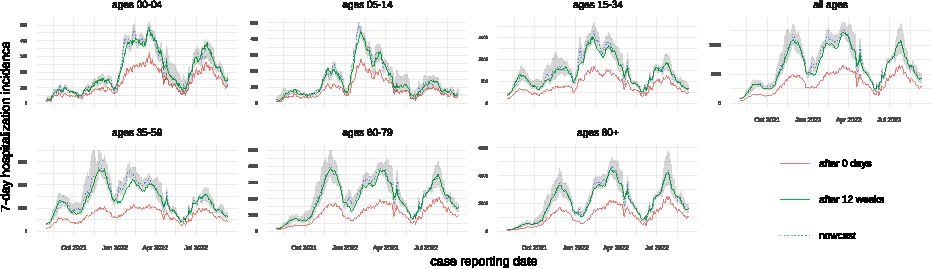
\includegraphics[width=\textwidth]{figures_tentative/delays_in_reporting-1.pdf} 

}

\caption{\textbf{TODO: redo figure with final model}Germany's $7$-day hospitalisation incidence changes due to various delays such as time to hospitalisation and delays in reporting. This figure shows the extent of these delays: incidences reported at the present date (red lines) severely underestimate the hospitalisation incidence (green solid lines) that is reported after $3$ months. Our nowcasting model (blue dotted lines, 95\% prediction intervals in shaded gray) deals with this problem by predicting the hospitalisation incidence based on past cases and their delays to hospitalisation.}\label{fig:delays_in_reporting}
\end{figure}

The origin of nowcasting lie in accounting for incurred, but not reported claims in the actuarial sciences \citep{Kaminsky1987Prediction}, delays in reporting for AIDS \citep{Zeger1989Statistical,Lawless1994Adjustments} and other infectious diseases \citep{Farrington1996Statistical}. Popular statistical approaches include methods from survival analysis \citep{Lawless1994Adjustments} and generalized linear regression \citep{Zeger1989Statistical}. In the survial analysis setting one commonly models the reverse time discrete hazard parametrically and assumes multinomial sampling of the final number of cases, potentially accounting for overdispersion. This has been studied with frequentist \citep{Midthune2005Modeling} and Bayesian \citep{Hohle2014Bayesian,AnDerHeiden2020Schatzung} methods. The generalized linear regression approach has origins in the chain ladder model from actuarial sciences \citep{Renshaw1998Stochastic} and models the observed counts in the reporting triangle by a Poisson or negative binomial distribution.
For both approaches, available covariates can be incorporated in a straightforward way. In the setting of real-time nowcasting, it is often beneficial to incorporate epidemic dynamics into the model, this can be achieved by splines \citep{Hohle2014Bayesian,vandeKassteele2019Nowcasting} or by a latent process of infections \citep{McGough2020Nowcasting}.

Nowcasting methods have wide application in accouting for reporting delays \citep{Midthune2005Modeling}, early outbreak detection \citep{Salmon2015Bayesian,Bastos2019Modelling}, and, in the recent COVID-19 epidemic, improving real-time monitoring of epidemic outbreaks \citep{AnDerHeiden2020Schatzung,Gunther2021Nowcasting,Schneble2021Nowcasting,Akhmetzhanov2021Estimation}. Evaluating a forecasting model in a real-time public health setting is advantageous as it avoid hindsight bias \citep{Desai2019Realtime}, however nowcasting approach may have difficulties with bias and properly calibrated uncertainty if used in a real-time setting. This includes rapidly changing dynamics \citep{Gunther2021Nowcasting,vandeKassteele2019Nowcasting}, both of the delay distribution and the underlying epidemic, retrospective changes in data \citep{Midthune2005Modeling} and long delays with few observed cases \citep{Noufaily2015Modelling}. 

To avoid the aforementioned hindsight bias one can make their predictions publicly available in real-time \citep{Ray2020Ensemble,Bracher2021Preregistered}. For the hospitalisations in Germany, we have participated in the German COVID-19 NowcastHub \citep{2022Nowcasts} since November 2021 where nowcasts are available in a public Github repository \citep{2022Hospitalization} with the ``ILM-prop'' model. The ideas, especially the model and the ``double-weekday effect'', discussed this section are based on this model. However, the ``ILM-prop'' model is based on simple point estimates for the proportion of hospitalisations per reported case, neglecting regularization over time. In this thesis we extend this model to the \gls{ssm} setting of this thesis and investigate if the increased model complexity results in improved performance. In particular, we want to reduce computation time, as the previous model quantified uncertainty by past model performance, which requires running the model many times. If prediction uncertainty is based on predicting future observations in a \acrshort{ssm}, we can reduce computation time drastically. However, this is only worthwhile, if the predictive performance is comparable to the computationally more intensive model.

%\subsection{Data}
To predict the number of hospitalisations we consider the reporting process of both reported COVID-19 cases and reported hospitalisations. Recall that the reporting date of a COVID-19 case is shared for both the case and its hospitalisation, i.e.~the case and hospitalisation are linked through this date.

As hospitalisations are only available as \(7\)-day rolling sums, we use \(7\)-day rolling sums for daily reported incidences as well. To avoid dealing with the double weekday effect of both reporting date of the case and reporting date of the hospitalisation (see \cref{fig:double_weekday_effect}) we divide the future hospitalisations we wish to predict into chunks of one week, which gets rid of the weekday effect for the hospitalisations. This is depicted in \cref{fig:reporting_triangle}. Our prediction of each of these weekly chunks then consists of the fraction of hospitalisations of reported cases in the past.

We use the publicly available data from the \acrshort{rki} discussed in \Cref{sec:data} on daily reported COVID-19 cases \citep{RobertKoch-Institut2024SARSCoV2} and weekly reported hospitalizations \citep{RobertKoch-Institut2024COVID19Hospitalisierungen}. Both datasets are updated daily.

Recall from \Cref{sec:data} that COVID-19 cases are described by their date of reporting, and are subject to reporting delay and hospitalizations are reported by the \textit{reporting date of the associated case}, and are subject to delay as well. As the date of symptom onset is not known for a substantial amount of incident cases, and is not reported for hospitalized cases, we focus our analysis on the date of reporting.


\begin{figure}
    \resizebox{\textwidth}{!}{%
        % Created by tikzDevice version 0.12.6 on 2025-08-10 11:58:55
% !TEX encoding = UTF-8 Unicode
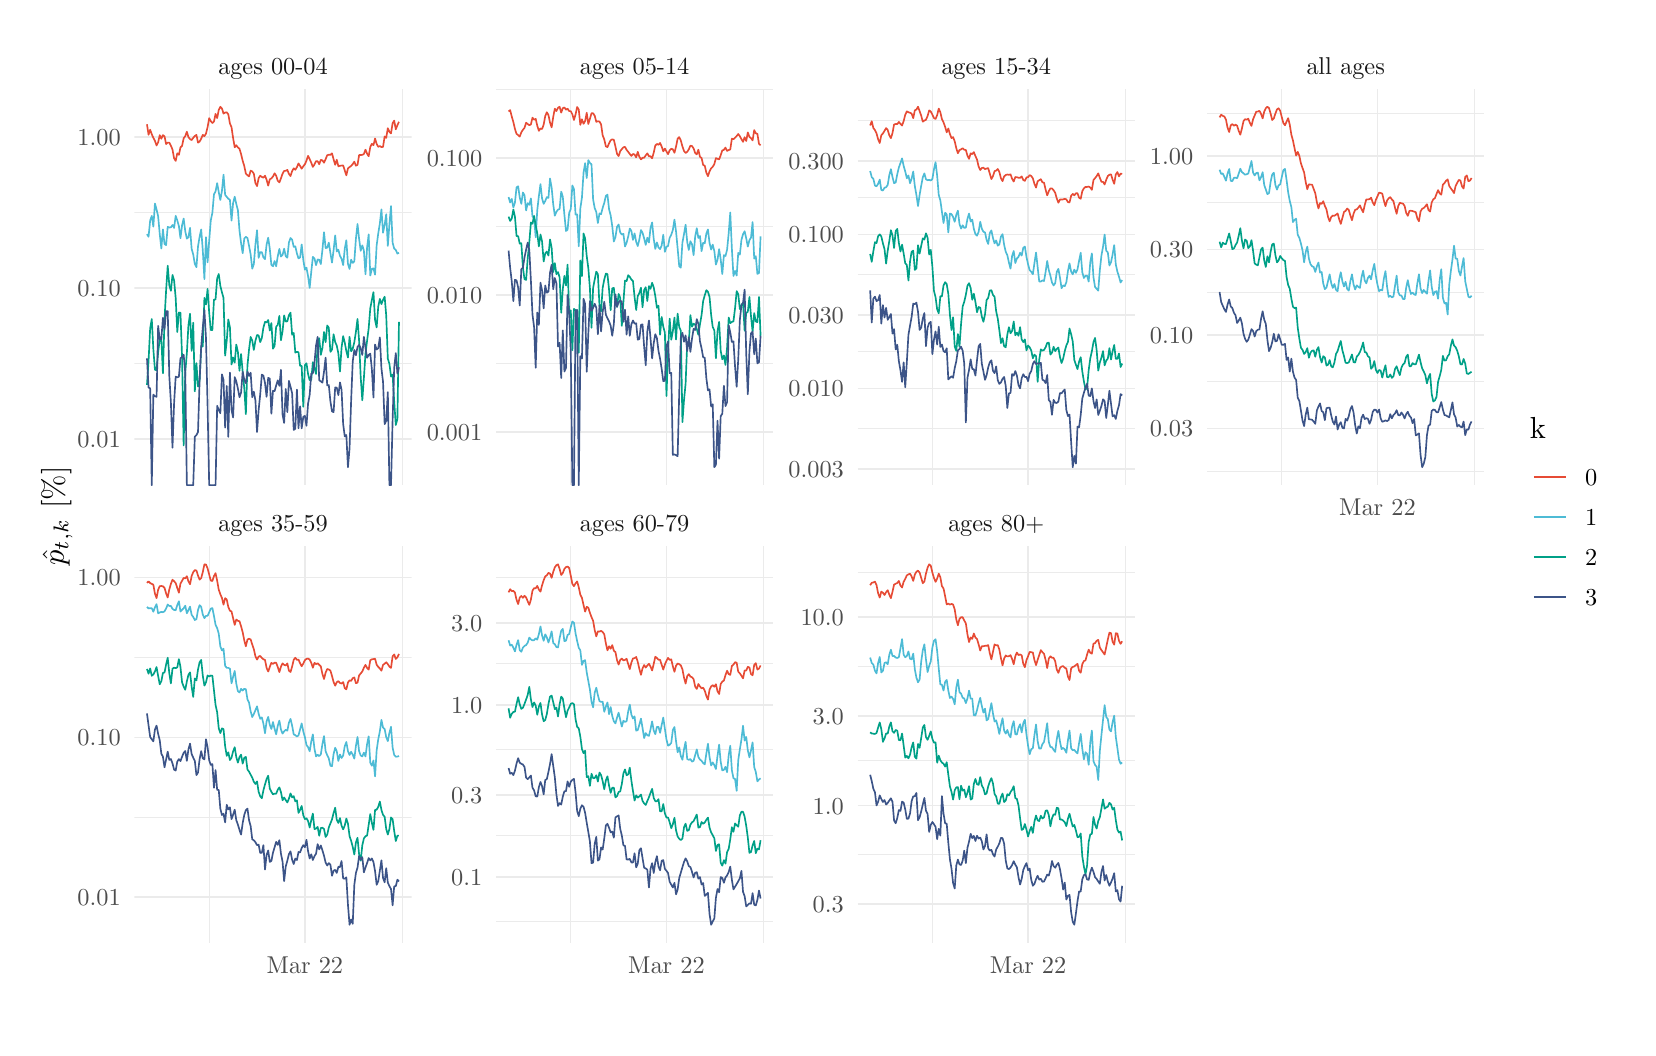
\begin{tikzpicture}[x=1pt,y=1pt]
\definecolor{fillColor}{RGB}{255,255,255}
\path[use as bounding box,fill=fillColor,fill opacity=0.00] (0,0) rectangle (578.16,361.35);
\begin{scope}
\path[clip] ( 38.56,196.02) rectangle (138.73,339.28);
\definecolor{drawColor}{gray}{0.92}

\path[draw=drawColor,line width= 0.3pt,line join=round] ( 38.56,240.06) --
	(138.73,240.06);

\path[draw=drawColor,line width= 0.3pt,line join=round] ( 38.56,294.53) --
	(138.73,294.53);

\path[draw=drawColor,line width= 0.3pt,line join=round] ( 65.59,196.02) --
	( 65.59,339.28);

\path[draw=drawColor,line width= 0.3pt,line join=round] (135.33,196.02) --
	(135.33,339.28);

\path[draw=drawColor,line width= 0.6pt,line join=round] ( 38.56,212.83) --
	(138.73,212.83);

\path[draw=drawColor,line width= 0.6pt,line join=round] ( 38.56,267.30) --
	(138.73,267.30);

\path[draw=drawColor,line width= 0.6pt,line join=round] ( 38.56,321.76) --
	(138.73,321.76);

\path[draw=drawColor,line width= 0.6pt,line join=round] (100.17,196.02) --
	(100.17,339.28);
\definecolor{drawColor}{RGB}{230,75,53}

\path[draw=drawColor,line width= 0.6pt,line join=round] ( 43.11,326.42) --
	( 43.68,322.65) --
	( 44.26,324.47) --
	( 44.84,322.84) --
	( 45.41,321.54) --
	( 45.99,320.46) --
	( 46.57,318.79) --
	( 47.14,319.90) --
	( 47.72,322.51) --
	( 48.30,321.21) --
	( 48.87,322.51) --
	( 49.45,322.07) --
	( 50.02,319.29) --
	( 50.60,319.82) --
	( 51.18,319.80) --
	( 51.75,318.72) --
	( 52.33,317.30) --
	( 52.91,314.14) --
	( 53.48,313.20) --
	( 54.06,315.96) --
	( 54.64,315.39) --
	( 55.21,318.07) --
	( 55.79,318.64) --
	( 56.36,321.36) --
	( 56.94,322.15) --
	( 57.52,323.77) --
	( 58.09,321.79) --
	( 58.67,321.09) --
	( 59.25,320.72) --
	( 59.82,321.54) --
	( 60.40,322.22) --
	( 60.98,322.59) --
	( 61.55,319.78) --
	( 62.13,320.20) --
	( 62.70,321.23) --
	( 63.28,322.62) --
	( 63.86,322.14) --
	( 64.43,323.04) --
	( 65.01,325.41) --
	( 65.59,328.64) --
	( 66.16,327.58) --
	( 66.74,326.91) --
	( 67.32,327.44) --
	( 67.89,330.19) --
	( 68.47,328.67) --
	( 69.04,331.60) --
	( 69.62,332.77) --
	( 70.20,332.11) --
	( 70.77,330.32) --
	( 71.35,330.67) --
	( 71.93,330.76) --
	( 72.50,330.04) --
	( 73.08,326.74) --
	( 73.66,325.38) --
	( 74.23,321.47) --
	( 74.81,318.13) --
	( 75.38,318.85) --
	( 75.96,318.07) --
	( 76.54,317.58) --
	( 77.11,315.67) --
	( 77.69,313.24) --
	( 78.27,311.35) --
	( 78.84,308.61) --
	( 79.42,308.04) --
	( 79.99,307.61) --
	( 80.57,309.68) --
	( 81.15,309.41) --
	( 81.72,308.58) --
	( 82.30,305.19) --
	( 82.88,304.10) --
	( 83.45,306.96) --
	( 84.03,307.85) --
	( 84.61,307.41) --
	( 85.18,307.15) --
	( 85.76,307.85) --
	( 86.33,306.41) --
	( 86.91,304.27) --
	( 87.49,306.55) --
	( 88.06,306.87) --
	( 88.64,307.58) --
	( 89.22,308.72) --
	( 89.79,307.84) --
	( 90.37,306.02) --
	( 90.95,305.43) --
	( 91.52,306.91) --
	( 92.10,308.57) --
	( 92.67,309.58) --
	( 93.25,309.62) --
	( 93.83,309.95) --
	( 94.40,308.53) --
	( 94.98,307.74) --
	( 95.56,309.51) --
	( 96.13,310.52) --
	( 96.71,309.99) --
	( 97.29,310.94) --
	( 97.86,312.29) --
	( 98.44,311.37) --
	( 99.01,310.38) --
	( 99.59,311.28) --
	(100.17,311.97) --
	(100.74,313.28) --
	(101.32,315.02) --
	(101.90,313.83) --
	(102.47,312.56) --
	(103.05,311.04) --
	(103.63,311.93) --
	(104.20,313.12) --
	(104.78,313.08) --
	(105.35,312.00) --
	(105.93,313.59) --
	(106.51,313.38) --
	(107.08,312.55) --
	(107.66,313.83) --
	(108.24,315.26) --
	(108.81,315.42) --
	(109.39,315.40) --
	(109.97,315.94) --
	(110.54,313.77) --
	(111.12,311.80) --
	(111.69,313.62) --
	(112.27,311.26) --
	(112.85,311.44) --
	(113.42,311.51) --
	(114.00,311.58) --
	(114.58,309.76) --
	(115.15,307.98) --
	(115.73,310.50) --
	(116.31,310.97) --
	(116.88,311.39) --
	(117.46,312.05) --
	(118.03,312.94) --
	(118.61,311.46) --
	(119.19,311.77) --
	(119.76,315.31) --
	(120.34,315.34) --
	(120.92,315.39) --
	(121.49,315.70) --
	(122.07,317.25) --
	(122.65,315.80) --
	(123.22,314.90) --
	(123.80,318.22) --
	(124.37,319.38) --
	(124.95,318.88) --
	(125.53,321.29) --
	(126.10,319.33) --
	(126.68,318.29) --
	(127.26,318.59) --
	(127.83,318.17) --
	(128.41,318.31) --
	(128.99,322.03) --
	(129.56,321.54) --
	(130.14,325.00) --
	(130.71,323.74) --
	(131.29,323.14) --
	(131.87,326.81) --
	(132.44,327.76) --
	(133.02,324.60) --
	(133.60,326.13) --
	(134.17,327.32);
\definecolor{drawColor}{RGB}{77,187,213}

\path[draw=drawColor,line width= 0.6pt,line join=round] ( 43.11,286.75) --
	( 43.68,285.80) --
	( 44.26,291.67) --
	( 44.84,293.33) --
	( 45.41,289.45) --
	( 45.99,297.81) --
	( 46.57,295.68) --
	( 47.14,293.19) --
	( 47.72,286.83) --
	( 48.30,281.54) --
	( 48.87,288.44) --
	( 49.45,283.15) --
	( 50.02,282.77) --
	( 50.60,289.38) --
	( 51.18,289.14) --
	( 51.75,289.20) --
	( 52.33,290.03) --
	( 52.91,288.98) --
	( 53.48,293.36) --
	( 54.06,291.70) --
	( 54.64,289.67) --
	( 55.21,285.28) --
	( 55.79,289.93) --
	( 56.36,292.37) --
	( 56.94,287.82) --
	( 57.52,285.09) --
	( 58.09,285.65) --
	( 58.67,288.99) --
	( 59.25,281.43) --
	( 59.82,279.39) --
	( 60.40,275.96) --
	( 60.98,274.81) --
	( 61.55,282.28) --
	( 62.13,285.82) --
	( 62.70,288.44) --
	( 63.28,280.86) --
	( 63.86,270.49) --
	( 64.43,285.66) --
	( 65.01,276.55) --
	( 65.59,284.37) --
	( 66.16,291.68) --
	( 66.74,294.45) --
	( 67.32,301.14) --
	( 67.89,302.17) --
	( 68.47,305.17) --
	( 69.04,301.97) --
	( 69.62,299.08) --
	( 70.20,302.38) --
	( 70.77,308.24) --
	( 71.35,300.94) --
	( 71.93,300.21) --
	( 72.50,299.53) --
	( 73.08,299.12) --
	( 73.66,291.62) --
	( 74.23,297.99) --
	( 74.81,300.27) --
	( 75.38,297.65) --
	( 75.96,295.41) --
	( 76.54,288.02) --
	( 77.11,283.49) --
	( 77.69,279.86) --
	( 78.27,285.14) --
	( 78.84,285.77) --
	( 79.42,285.34) --
	( 79.99,282.50) --
	( 80.57,279.40) --
	( 81.15,274.26) --
	( 81.72,275.88) --
	( 82.30,283.03) --
	( 82.88,288.14) --
	( 83.45,278.18) --
	( 84.03,280.23) --
	( 84.61,280.24) --
	( 85.18,278.32) --
	( 85.76,277.71) --
	( 86.33,282.96) --
	( 86.91,285.45) --
	( 87.49,281.39) --
	( 88.06,275.61) --
	( 88.64,275.14) --
	( 89.22,277.01) --
	( 89.79,275.13) --
	( 90.37,278.79) --
	( 90.95,281.38) --
	( 91.52,278.64) --
	( 92.10,279.20) --
	( 92.67,281.49) --
	( 93.25,278.78) --
	( 93.83,278.22) --
	( 94.40,283.70) --
	( 94.98,285.35) --
	( 95.56,284.73) --
	( 96.13,282.16) --
	( 96.71,282.32) --
	( 97.29,279.76) --
	( 97.86,277.96) --
	( 98.44,278.32) --
	( 99.01,283.01) --
	( 99.59,277.44) --
	(100.17,273.90) --
	(100.74,274.62) --
	(101.32,271.54) --
	(101.90,267.31) --
	(102.47,273.07) --
	(103.05,278.52) --
	(103.63,277.97) --
	(104.20,275.54) --
	(104.78,277.59) --
	(105.35,277.49) --
	(105.93,275.92) --
	(106.51,281.06) --
	(107.08,287.44) --
	(107.66,281.72) --
	(108.24,281.83) --
	(108.81,283.66) --
	(109.39,279.93) --
	(109.97,276.45) --
	(110.54,280.91) --
	(111.12,286.29) --
	(111.69,280.46) --
	(112.27,281.10) --
	(112.85,278.88) --
	(113.42,277.86) --
	(114.00,275.54) --
	(114.58,281.47) --
	(115.15,284.54) --
	(115.73,276.00) --
	(116.31,274.15) --
	(116.88,277.51) --
	(117.46,276.34) --
	(118.03,276.94) --
	(118.61,285.10) --
	(119.19,290.39) --
	(119.76,285.06) --
	(120.34,280.72) --
	(120.92,282.69) --
	(121.49,280.79) --
	(122.07,272.24) --
	(122.65,281.94) --
	(123.22,286.65) --
	(123.80,271.78) --
	(124.37,274.19) --
	(124.95,274.40) --
	(125.53,272.10) --
	(126.10,282.65) --
	(126.68,287.02) --
	(127.26,290.62) --
	(127.83,295.68) --
	(128.41,287.25) --
	(128.99,290.10) --
	(129.56,293.93) --
	(130.14,282.47) --
	(130.71,290.26) --
	(131.29,296.87) --
	(131.87,283.65) --
	(132.44,281.52) --
	(133.02,281.03) --
	(133.60,279.70) --
	(134.17,280.01);
\definecolor{drawColor}{RGB}{0,160,135}

\path[draw=drawColor,line width= 0.6pt,line join=round] ( 43.11,232.28) --
	( 43.68,240.92) --
	( 44.26,252.68) --
	( 44.84,256.06) --
	( 45.41,245.17) --
	( 45.99,237.75) --
	( 46.57,237.56) --
	( 47.14,244.00) --
	( 47.72,248.76) --
	( 48.30,248.74) --
	( 48.87,236.46) --
	( 49.45,256.06) --
	( 50.02,266.38) --
	( 50.60,275.32) --
	( 51.18,268.27) --
	( 51.75,266.27) --
	( 52.33,272.00) --
	( 52.91,270.00) --
	( 53.48,263.72) --
	( 54.06,251.38) --
	( 54.64,258.40) --
	( 55.21,258.33) --
	( 55.79,242.27) --
	( 56.36,210.39) --
	( 56.94,236.74) --
	( 57.52,243.72) --
	( 58.09,253.86) --
	( 58.67,257.96) --
	( 59.25,244.58) --
	( 59.82,254.76) --
	( 60.40,229.93) --
	( 60.98,240.13) --
	( 61.55,231.66) --
	( 62.13,233.84) --
	( 62.70,246.06) --
	( 63.28,246.17) --
	( 63.86,263.69) --
	( 64.43,261.30) --
	( 65.01,266.96) --
	( 65.59,258.38) --
	( 66.16,252.08) --
	( 66.74,252.07) --
	( 67.32,263.07) --
	( 67.89,263.17) --
	( 68.47,270.75) --
	( 69.04,272.33) --
	( 69.62,268.04) --
	( 70.20,265.70) --
	( 70.77,263.70) --
	( 71.35,242.83) --
	( 71.93,248.24) --
	( 72.50,255.87) --
	( 73.08,253.09) --
	( 73.66,239.65) --
	( 74.23,242.15) --
	( 74.81,240.34) --
	( 75.38,246.83) --
	( 75.96,244.20) --
	( 76.54,237.40) --
	( 77.11,243.41) --
	( 77.69,236.99) --
	( 78.27,231.02) --
	( 78.84,221.72) --
	( 79.42,239.31) --
	( 79.99,245.07) --
	( 80.57,249.59) --
	( 81.15,248.27) --
	( 81.72,244.90) --
	( 82.30,248.26) --
	( 82.88,250.29) --
	( 83.45,250.14) --
	( 84.03,247.73) --
	( 84.61,249.20) --
	( 85.18,252.97) --
	( 85.76,255.05) --
	( 86.33,254.82) --
	( 86.91,255.70) --
	( 87.49,251.89) --
	( 88.06,254.62) --
	( 88.64,245.33) --
	( 89.22,246.38) --
	( 89.79,253.28) --
	( 90.37,253.96) --
	( 90.95,257.19) --
	( 91.52,248.40) --
	( 92.10,251.68) --
	( 92.67,257.36) --
	( 93.25,255.16) --
	( 93.83,255.23) --
	( 94.40,257.45) --
	( 94.98,258.37) --
	( 95.56,250.38) --
	( 96.13,251.04) --
	( 96.71,243.95) --
	( 97.29,244.18) --
	( 97.86,244.08) --
	( 98.44,239.18) --
	( 99.01,239.15) --
	( 99.59,224.36) --
	(100.17,239.36) --
	(100.74,240.08) --
	(101.32,236.20) --
	(101.90,233.94) --
	(102.47,234.08) --
	(103.05,240.45) --
	(103.63,238.37) --
	(104.20,236.22) --
	(104.78,246.98) --
	(105.35,249.14) --
	(105.93,243.12) --
	(106.51,245.64) --
	(107.08,251.39) --
	(107.66,247.71) --
	(108.24,253.73) --
	(108.81,252.92) --
	(109.39,244.19) --
	(109.97,245.01) --
	(110.54,250.55) --
	(111.12,247.75) --
	(111.69,246.45) --
	(112.27,243.59) --
	(112.85,237.11) --
	(113.42,245.69) --
	(114.00,249.90) --
	(114.58,247.58) --
	(115.15,244.46) --
	(115.73,242.13) --
	(116.31,249.64) --
	(116.88,244.37) --
	(117.46,245.36) --
	(118.03,247.69) --
	(118.61,251.44) --
	(119.19,256.10) --
	(119.76,248.20) --
	(120.34,235.07) --
	(120.92,226.70) --
	(121.49,234.76) --
	(122.07,243.55) --
	(122.65,248.25) --
	(123.22,252.70) --
	(123.80,259.94) --
	(124.37,262.95) --
	(124.95,265.78) --
	(125.53,255.71) --
	(126.10,253.02) --
	(126.68,260.58) --
	(127.26,263.35) --
	(127.83,261.45) --
	(128.41,263.02) --
	(128.99,264.11) --
	(129.56,257.33) --
	(130.14,241.72) --
	(130.71,239.92) --
	(131.29,235.30) --
	(131.87,235.99) --
	(132.44,226.28) --
	(133.02,217.77) --
	(133.60,219.96) --
	(134.17,255.03);
\definecolor{drawColor}{RGB}{60,84,136}

\path[draw=drawColor,line width= 0.6pt,line join=round] ( 43.11,241.87) --
	( 43.68,231.33) --
	( 44.26,231.00) --
	( 44.84,196.02) --
	( 45.41,228.77) --
	( 45.99,228.16) --
	( 46.57,227.97) --
	( 47.14,253.59) --
	( 47.72,248.76) --
	( 48.30,248.74) --
	( 48.87,256.51) --
	( 49.45,252.42) --
	( 50.02,258.84) --
	( 50.60,258.92) --
	( 51.18,235.47) --
	( 51.75,225.94) --
	( 52.33,209.58) --
	( 52.91,225.73) --
	( 53.48,235.24) --
	( 54.06,234.98) --
	( 54.64,235.20) --
	( 55.21,241.93) --
	( 55.79,242.27) --
	( 56.36,243.18) --
	( 56.94,236.74) --
	( 57.52,196.02) --
	( 58.09,196.02) --
	( 58.67,196.02) --
	( 59.25,196.02) --
	( 59.82,196.02) --
	( 60.40,213.53) --
	( 60.98,214.14) --
	( 61.55,215.26) --
	( 62.13,233.84) --
	( 62.70,246.06) --
	( 63.28,252.98) --
	( 63.86,259.38) --
	( 64.43,249.22) --
	( 65.01,224.58) --
	( 65.59,196.02) --
	( 66.16,196.02) --
	( 66.74,196.02) --
	( 67.32,196.02) --
	( 67.89,196.02) --
	( 68.47,224.72) --
	( 69.04,223.15) --
	( 69.62,222.02) --
	( 70.20,236.07) --
	( 70.77,234.07) --
	( 71.35,216.84) --
	( 71.93,231.84) --
	( 72.50,213.49) --
	( 73.08,236.69) --
	( 73.66,223.25) --
	( 74.23,220.48) --
	( 74.81,235.06) --
	( 75.38,233.59) --
	( 75.96,230.96) --
	( 76.54,227.81) --
	( 77.11,229.50) --
	( 77.69,236.99) --
	( 78.27,234.17) --
	( 78.84,232.83) --
	( 79.42,237.06) --
	( 79.99,235.48) --
	( 80.57,236.67) --
	( 81.15,227.81) --
	( 81.72,229.85) --
	( 82.30,226.58) --
	( 82.88,215.24) --
	( 83.45,223.05) --
	( 84.03,228.85) --
	( 84.61,235.97) --
	( 85.18,235.61) --
	( 85.76,232.95) --
	( 86.33,227.97) --
	( 86.91,234.83) --
	( 87.49,234.53) --
	( 88.06,221.83) --
	( 88.64,230.15) --
	( 89.22,229.99) --
	( 89.79,232.04) --
	( 90.37,233.91) --
	( 90.95,231.93) --
	( 91.52,237.71) --
	( 92.10,221.57) --
	( 92.67,218.51) --
	( 93.25,230.80) --
	( 93.83,222.44) --
	( 94.40,233.72) --
	( 94.98,231.60) --
	( 95.56,229.24) --
	( 96.13,215.99) --
	( 96.71,216.44) --
	( 97.29,230.57) --
	( 97.86,216.57) --
	( 98.44,224.54) --
	( 99.01,216.55) --
	( 99.59,220.72) --
	(100.17,221.07) --
	(100.74,217.48) --
	(101.32,225.51) --
	(101.90,228.66) --
	(102.47,236.33) --
	(103.05,236.50) --
	(103.63,240.26) --
	(104.20,246.51) --
	(104.78,249.61) --
	(105.35,233.96) --
	(105.93,233.53) --
	(106.51,233.09) --
	(107.08,237.05) --
	(107.66,242.12) --
	(108.24,232.06) --
	(108.81,232.21) --
	(109.39,226.36) --
	(109.97,222.67) --
	(110.54,222.41) --
	(111.12,231.35) --
	(111.69,231.27) --
	(112.27,228.55) --
	(112.85,233.16) --
	(113.42,230.51) --
	(114.00,218.11) --
	(114.58,213.63) --
	(115.15,214.16) --
	(115.73,202.53) --
	(116.31,209.32) --
	(116.88,226.54) --
	(117.46,240.77) --
	(118.03,244.90) --
	(118.61,243.00) --
	(119.19,245.99) --
	(119.76,246.68) --
	(120.34,245.52) --
	(120.92,243.09) --
	(121.49,249.63) --
	(122.07,245.61) --
	(122.65,242.05) --
	(123.22,243.11) --
	(123.80,243.54) --
	(124.37,237.97) --
	(124.95,227.71) --
	(125.53,246.84) --
	(126.10,245.06) --
	(126.68,245.53) --
	(127.26,249.45) --
	(127.83,238.25) --
	(128.41,233.38) --
	(128.99,218.08) --
	(129.56,219.26) --
	(130.14,229.64) --
	(130.71,196.02) --
	(131.29,196.02) --
	(131.87,219.59) --
	(132.44,238.36) --
	(133.02,243.76) --
	(133.60,236.35) --
	(134.17,238.63);
\end{scope}
\begin{scope}
\path[clip] ( 38.56, 30.69) rectangle (138.73,173.95);
\definecolor{drawColor}{gray}{0.92}

\path[draw=drawColor,line width= 0.3pt,line join=round] ( 38.56, 76.00) --
	(138.73, 76.00);

\path[draw=drawColor,line width= 0.3pt,line join=round] ( 38.56,133.76) --
	(138.73,133.76);

\path[draw=drawColor,line width= 0.3pt,line join=round] ( 65.59, 30.69) --
	( 65.59,173.95);

\path[draw=drawColor,line width= 0.3pt,line join=round] (135.33, 30.69) --
	(135.33,173.95);

\path[draw=drawColor,line width= 0.6pt,line join=round] ( 38.56, 47.12) --
	(138.73, 47.12);

\path[draw=drawColor,line width= 0.6pt,line join=round] ( 38.56,104.88) --
	(138.73,104.88);

\path[draw=drawColor,line width= 0.6pt,line join=round] ( 38.56,162.64) --
	(138.73,162.64);

\path[draw=drawColor,line width= 0.6pt,line join=round] (100.17, 30.69) --
	(100.17,173.95);
\definecolor{drawColor}{RGB}{230,75,53}

\path[draw=drawColor,line width= 0.6pt,line join=round] ( 43.11,160.74) --
	( 43.68,161.27) --
	( 44.26,160.66) --
	( 44.84,160.38) --
	( 45.41,160.06) --
	( 45.99,156.84) --
	( 46.57,155.23) --
	( 47.14,158.24) --
	( 47.72,159.52) --
	( 48.30,159.60) --
	( 48.87,159.48) --
	( 49.45,158.93) --
	( 50.02,156.93) --
	( 50.60,155.45) --
	( 51.18,158.37) --
	( 51.75,160.36) --
	( 52.33,161.86) --
	( 52.91,161.33) --
	( 53.48,160.64) --
	( 54.06,158.88) --
	( 54.64,157.17) --
	( 55.21,160.48) --
	( 55.79,161.47) --
	( 56.36,162.53) --
	( 56.94,162.33) --
	( 57.52,163.13) --
	( 58.09,161.30) --
	( 58.67,160.23) --
	( 59.25,163.22) --
	( 59.82,164.60) --
	( 60.40,165.33) --
	( 60.98,165.22) --
	( 61.55,163.36) --
	( 62.13,161.88) --
	( 62.70,162.44) --
	( 63.28,164.63) --
	( 63.86,167.43) --
	( 64.43,167.35) --
	( 65.01,165.96) --
	( 65.59,163.73) --
	( 66.16,161.56) --
	( 66.74,161.40) --
	( 67.32,163.18) --
	( 67.89,164.22) --
	( 68.47,161.51) --
	( 69.04,158.28) --
	( 69.62,156.61) --
	( 70.20,155.29) --
	( 70.77,152.86) --
	( 71.35,155.20) --
	( 71.93,154.71) --
	( 72.50,152.02) --
	( 73.08,150.66) --
	( 73.66,150.42) --
	( 74.23,147.96) --
	( 74.81,145.55) --
	( 75.38,147.49) --
	( 75.96,147.02) --
	( 76.54,146.85) --
	( 77.11,145.06) --
	( 77.69,142.90) --
	( 78.27,139.92) --
	( 78.84,137.82) --
	( 79.42,140.27) --
	( 79.99,140.54) --
	( 80.57,140.28) --
	( 81.15,138.45) --
	( 81.72,136.78) --
	( 82.30,134.20) --
	( 82.88,133.01) --
	( 83.45,134.10) --
	( 84.03,134.32) --
	( 84.61,133.61) --
	( 85.18,133.11) --
	( 85.76,132.89) --
	( 86.33,129.99) --
	( 86.91,128.68) --
	( 87.49,130.42) --
	( 88.06,131.80) --
	( 88.64,131.47) --
	( 89.22,131.89) --
	( 89.79,131.85) --
	( 90.37,130.30) --
	( 90.95,128.48) --
	( 91.52,130.43) --
	( 92.10,131.65) --
	( 92.67,131.12) --
	( 93.25,130.87) --
	( 93.83,131.63) --
	( 94.40,129.01) --
	( 94.98,128.52) --
	( 95.56,130.49) --
	( 96.13,132.93) --
	( 96.71,133.67) --
	( 97.29,132.93) --
	( 97.86,133.01) --
	( 98.44,131.66) --
	( 99.01,130.60) --
	( 99.59,131.56) --
	(100.17,132.77) --
	(100.74,133.25) --
	(101.32,133.38) --
	(101.90,133.02) --
	(102.47,131.89) --
	(103.05,130.07) --
	(103.63,131.82) --
	(104.20,131.37) --
	(104.78,131.68) --
	(105.35,131.10) --
	(105.93,130.55) --
	(106.51,127.78) --
	(107.08,125.99) --
	(107.66,128.27) --
	(108.24,129.61) --
	(108.81,129.43) --
	(109.39,129.03) --
	(109.97,127.08) --
	(110.54,124.91) --
	(111.12,123.57) --
	(111.69,124.85) --
	(112.27,125.22) --
	(112.85,124.54) --
	(113.42,124.35) --
	(114.00,124.87) --
	(114.58,122.68) --
	(115.15,122.25) --
	(115.73,124.71) --
	(116.31,125.52) --
	(116.88,125.31) --
	(117.46,126.31) --
	(118.03,126.54) --
	(118.61,124.47) --
	(119.19,124.68) --
	(119.76,127.30) --
	(120.34,127.98) --
	(120.92,128.72) --
	(121.49,130.06) --
	(122.07,131.08) --
	(122.65,129.99) --
	(123.22,129.38) --
	(123.80,132.78) --
	(124.37,133.10) --
	(124.95,133.19) --
	(125.53,133.31) --
	(126.10,131.15) --
	(126.68,130.37) --
	(127.26,129.79) --
	(127.83,128.99) --
	(128.41,131.08) --
	(128.99,131.51) --
	(129.56,132.04) --
	(130.14,131.37) --
	(130.71,130.46) --
	(131.29,130.00) --
	(131.87,134.19) --
	(132.44,134.86) --
	(133.02,133.22) --
	(133.60,133.85) --
	(134.17,135.05);
\definecolor{drawColor}{RGB}{77,187,213}

\path[draw=drawColor,line width= 0.6pt,line join=round] ( 43.11,152.06) --
	( 43.68,151.49) --
	( 44.26,151.57) --
	( 44.84,151.58) --
	( 45.41,150.30) --
	( 45.99,151.91) --
	( 46.57,153.03) --
	( 47.14,149.72) --
	( 47.72,150.03) --
	( 48.30,150.26) --
	( 48.87,150.12) --
	( 49.45,150.44) --
	( 50.02,151.47) --
	( 50.60,152.90) --
	( 51.18,152.39) --
	( 51.75,152.40) --
	( 52.33,151.34) --
	( 52.91,150.95) --
	( 53.48,150.84) --
	( 54.06,152.72) --
	( 54.64,154.07) --
	( 55.21,150.36) --
	( 55.79,151.00) --
	( 56.36,151.54) --
	( 56.94,152.47) --
	( 57.52,149.74) --
	( 58.09,150.90) --
	( 58.67,152.12) --
	( 59.25,149.15) --
	( 59.82,148.43) --
	( 60.40,147.30) --
	( 60.98,147.61) --
	( 61.55,150.93) --
	( 62.13,152.66) --
	( 62.70,152.05) --
	( 63.28,149.26) --
	( 63.86,147.99) --
	( 64.43,148.80) --
	( 65.01,148.82) --
	( 65.59,150.09) --
	( 66.16,151.41) --
	( 66.74,151.63) --
	( 67.32,148.73) --
	( 67.89,145.59) --
	( 68.47,144.40) --
	( 69.04,142.36) --
	( 69.62,137.78) --
	( 70.20,136.32) --
	( 70.77,136.92) --
	( 71.35,130.77) --
	( 71.93,130.03) --
	( 72.50,130.02) --
	( 73.08,129.73) --
	( 73.66,124.44) --
	( 74.23,126.78) --
	( 74.81,128.92) --
	( 75.38,124.31) --
	( 75.96,121.59) --
	( 76.54,121.12) --
	( 77.11,122.44) --
	( 77.69,121.82) --
	( 78.27,122.44) --
	( 78.84,122.29) --
	( 79.42,118.64) --
	( 79.99,117.43) --
	( 80.57,114.31) --
	( 81.15,112.23) --
	( 81.72,113.33) --
	( 82.30,114.73) --
	( 82.88,116.12) --
	( 83.45,113.45) --
	( 84.03,111.62) --
	( 84.61,112.11) --
	( 85.18,109.87) --
	( 85.76,106.40) --
	( 86.33,110.68) --
	( 86.91,112.30) --
	( 87.49,109.42) --
	( 88.06,107.94) --
	( 88.64,110.45) --
	( 89.22,107.99) --
	( 89.79,105.99) --
	( 90.37,109.12) --
	( 90.95,110.96) --
	( 91.52,107.74) --
	( 92.10,106.27) --
	( 92.67,107.08) --
	( 93.25,107.62) --
	( 93.83,107.30) --
	( 94.40,110.22) --
	( 94.98,111.56) --
	( 95.56,109.13) --
	( 96.13,105.97) --
	( 96.71,105.70) --
	( 97.29,105.20) --
	( 97.86,105.62) --
	( 98.44,107.80) --
	( 99.01,109.94) --
	( 99.59,107.06) --
	(100.17,104.98) --
	(100.74,102.18) --
	(101.32,101.35) --
	(101.90, 99.89) --
	(102.47,103.37) --
	(103.05,105.99) --
	(103.63,100.77) --
	(104.20, 98.03) --
	(104.78, 98.61) --
	(105.35, 98.12) --
	(105.93, 98.76) --
	(106.51,102.54) --
	(107.08,105.35) --
	(107.66, 99.88) --
	(108.24, 98.45) --
	(108.81, 97.30) --
	(109.39, 94.65) --
	(109.97, 94.48) --
	(110.54, 98.89) --
	(111.12,101.15) --
	(111.69, 99.89) --
	(112.27, 96.37) --
	(112.85, 98.71) --
	(113.42, 97.47) --
	(114.00, 98.34) --
	(114.58,101.73) --
	(115.15,103.23) --
	(115.73, 99.93) --
	(116.31, 98.53) --
	(116.88, 99.69) --
	(117.46, 98.63) --
	(118.03, 97.22) --
	(118.61,101.81) --
	(119.19,105.05) --
	(119.76, 99.90) --
	(120.34, 98.34) --
	(120.92, 98.02) --
	(121.49, 99.38) --
	(122.07, 98.00) --
	(122.65,102.51) --
	(123.22,105.27) --
	(123.80, 95.74) --
	(124.37, 94.66) --
	(124.95, 96.56) --
	(125.53, 90.81) --
	(126.10,100.18) --
	(126.68,104.23) --
	(127.26,107.09) --
	(127.83,111.20) --
	(128.41,108.43) --
	(128.99,107.92) --
	(129.56,104.96) --
	(130.14,103.53) --
	(130.71,106.55) --
	(131.29,108.71) --
	(131.87,101.23) --
	(132.44, 98.55) --
	(133.02, 97.92) --
	(133.60, 97.94) --
	(134.17, 98.18);
\definecolor{drawColor}{RGB}{0,160,135}

\path[draw=drawColor,line width= 0.6pt,line join=round] ( 43.11,129.61) --
	( 43.68,127.90) --
	( 44.26,129.83) --
	( 44.84,127.16) --
	( 45.41,127.63) --
	( 45.99,128.71) --
	( 46.57,130.32) --
	( 47.14,127.09) --
	( 47.72,124.08) --
	( 48.30,125.19) --
	( 48.87,128.18) --
	( 49.45,128.35) --
	( 50.02,131.24) --
	( 50.60,133.65) --
	( 51.18,128.06) --
	( 51.75,124.38) --
	( 52.33,129.72) --
	( 52.91,130.08) --
	( 53.48,129.90) --
	( 54.06,130.19) --
	( 54.64,133.15) --
	( 55.21,130.34) --
	( 55.79,124.77) --
	( 56.36,123.27) --
	( 56.94,122.10) --
	( 57.52,125.12) --
	( 58.09,127.52) --
	( 58.67,128.39) --
	( 59.25,123.18) --
	( 59.82,119.52) --
	( 60.40,126.19) --
	( 60.98,125.49) --
	( 61.55,129.42) --
	( 62.13,132.07) --
	( 62.70,132.88) --
	( 63.28,127.18) --
	( 63.86,123.58) --
	( 64.43,124.79) --
	( 65.01,127.26) --
	( 65.59,126.88) --
	( 66.16,127.25) --
	( 66.74,127.16) --
	( 67.32,121.84) --
	( 67.89,116.61) --
	( 68.47,113.97) --
	( 69.04,108.25) --
	( 69.62,106.43) --
	( 70.20,108.15) --
	( 70.77,107.88) --
	( 71.35,101.72) --
	( 71.93, 98.22) --
	( 72.50, 99.51) --
	( 73.08, 96.71) --
	( 73.66, 97.58) --
	( 74.23, 99.82) --
	( 74.81,101.36) --
	( 75.38, 97.77) --
	( 75.96, 95.76) --
	( 76.54, 97.80) --
	( 77.11, 98.65) --
	( 77.69, 95.42) --
	( 78.27, 97.52) --
	( 78.84, 97.84) --
	( 79.42, 93.26) --
	( 79.99, 92.53) --
	( 80.57, 91.42) --
	( 81.15, 90.35) --
	( 81.72, 88.86) --
	( 82.30, 88.07) --
	( 82.88, 89.00) --
	( 83.45, 85.24) --
	( 84.03, 83.61) --
	( 84.61, 82.90) --
	( 85.18, 85.75) --
	( 85.76, 87.92) --
	( 86.33, 89.84) --
	( 86.91, 91.06) --
	( 87.49, 86.36) --
	( 88.06, 85.24) --
	( 88.64, 84.29) --
	( 89.22, 84.57) --
	( 89.79, 84.54) --
	( 90.37, 85.99) --
	( 90.95, 86.82) --
	( 91.52, 85.13) --
	( 92.10, 82.16) --
	( 92.67, 83.17) --
	( 93.25, 82.23) --
	( 93.83, 81.39) --
	( 94.40, 82.76) --
	( 94.98, 84.65) --
	( 95.56, 83.22) --
	( 96.13, 83.64) --
	( 96.71, 81.79) --
	( 97.29, 82.15) --
	( 97.86, 77.61) --
	( 98.44, 78.74) --
	( 99.01, 80.12) --
	( 99.59, 76.74) --
	(100.17, 75.38) --
	(100.74, 75.69) --
	(101.32, 74.66) --
	(101.90, 72.32) --
	(102.47, 75.01) --
	(103.05, 77.38) --
	(103.63, 71.77) --
	(104.20, 71.95) --
	(104.78, 72.55) --
	(105.35, 69.35) --
	(105.93, 72.15) --
	(106.51, 72.25) --
	(107.08, 71.78) --
	(107.66, 68.92) --
	(108.24, 69.77) --
	(108.81, 72.34) --
	(109.39, 73.80) --
	(109.97, 75.27) --
	(110.54, 77.56) --
	(111.12, 79.49) --
	(111.69, 75.07) --
	(112.27, 73.97) --
	(112.85, 75.73) --
	(113.42, 72.99) --
	(114.00, 71.65) --
	(114.58, 73.07) --
	(115.15, 75.57) --
	(115.73, 73.71) --
	(116.31, 69.22) --
	(116.88, 67.54) --
	(117.46, 65.31) --
	(118.03, 62.57) --
	(118.61, 66.92) --
	(119.19, 68.61) --
	(119.76, 62.64) --
	(120.34, 60.35) --
	(120.92, 65.92) --
	(121.49, 68.38) --
	(122.07, 69.18) --
	(122.65, 69.41) --
	(123.22, 73.28) --
	(123.80, 77.18) --
	(124.37, 74.04) --
	(124.95, 71.47) --
	(125.53, 78.70) --
	(126.10, 78.77) --
	(126.68, 79.81) --
	(127.26, 81.71) --
	(127.83, 78.68) --
	(128.41, 76.91) --
	(128.99, 76.20) --
	(129.56, 71.78) --
	(130.14, 69.78) --
	(130.71, 71.77) --
	(131.29, 75.96) --
	(131.87, 75.33) --
	(132.44, 71.10) --
	(133.02, 67.42) --
	(133.60, 69.39) --
	(134.17, 69.39);
\definecolor{drawColor}{RGB}{60,84,136}

\path[draw=drawColor,line width= 0.6pt,line join=round] ( 43.11,113.54) --
	( 43.68,109.24) --
	( 44.26,105.05) --
	( 44.84,104.21) --
	( 45.41,103.45) --
	( 45.99,107.74) --
	( 46.57,109.15) --
	( 47.14,106.21) --
	( 47.72,103.86) --
	( 48.30, 98.98) --
	( 48.87, 97.93) --
	( 49.45, 94.07) --
	( 50.02, 96.91) --
	( 50.60, 99.73) --
	( 51.18, 96.74) --
	( 51.75, 97.08) --
	( 52.33, 95.50) --
	( 52.91, 93.25) --
	( 53.48, 92.92) --
	( 54.06, 96.14) --
	( 54.64, 97.04) --
	( 55.21, 96.32) --
	( 55.79, 97.90) --
	( 56.36, 99.30) --
	( 56.94, 99.97) --
	( 57.52, 96.41) --
	( 58.09,100.59) --
	( 58.67,102.64) --
	( 59.25, 98.88) --
	( 59.82, 97.59) --
	( 60.40, 96.40) --
	( 60.98, 91.25) --
	( 61.55, 92.22) --
	( 62.13, 97.06) --
	( 62.70, 99.94) --
	( 63.28, 97.29) --
	( 63.86, 96.94) --
	( 64.43,104.21) --
	( 65.01,101.30) --
	( 65.59, 96.62) --
	( 66.16, 94.96) --
	( 66.74, 95.27) --
	( 67.32, 86.70) --
	( 67.89, 93.08) --
	( 68.47, 85.95) --
	( 69.04, 85.92) --
	( 69.62, 79.14) --
	( 70.20, 76.84) --
	( 70.77, 77.31) --
	( 71.35, 74.16) --
	( 71.93, 80.53) --
	( 72.50, 78.89) --
	( 73.08, 79.62) --
	( 73.66, 75.36) --
	( 74.23, 76.95) --
	( 74.81, 78.78) --
	( 75.38, 75.01) --
	( 75.96, 73.37) --
	( 76.54, 71.47) --
	( 77.11, 69.77) --
	( 77.69, 73.91) --
	( 78.27, 76.90) --
	( 78.84, 78.57) --
	( 79.42, 79.14) --
	( 79.99, 74.98) --
	( 80.57, 72.84) --
	( 81.15, 68.07) --
	( 81.72, 67.71) --
	( 82.30, 67.02) --
	( 82.88, 65.94) --
	( 83.45, 66.15) --
	( 84.03, 63.14) --
	( 84.61, 63.18) --
	( 85.18, 65.94) --
	( 85.76, 57.17) --
	( 86.33, 62.39) --
	( 86.91, 64.03) --
	( 87.49, 59.90) --
	( 88.06, 60.24) --
	( 88.64, 63.21) --
	( 89.22, 65.17) --
	( 89.79, 67.15) --
	( 90.37, 66.06) --
	( 90.95, 67.74) --
	( 91.52, 62.89) --
	( 92.10, 60.02) --
	( 92.67, 52.92) --
	( 93.25, 58.26) --
	( 93.83, 60.34) --
	( 94.40, 62.71) --
	( 94.98, 63.71) --
	( 95.56, 60.67) --
	( 96.13, 59.13) --
	( 96.71, 61.12) --
	( 97.29, 60.57) --
	( 97.86, 63.48) --
	( 98.44, 63.31) --
	( 99.01, 64.94) --
	( 99.59, 65.94) --
	(100.17, 65.21) --
	(100.74, 67.87) --
	(101.32, 63.78) --
	(101.90, 61.13) --
	(102.47, 62.64) --
	(103.05, 60.59) --
	(103.63, 61.97) --
	(104.20, 62.83) --
	(104.78, 66.31) --
	(105.35, 64.42) --
	(105.93, 65.85) --
	(106.51, 64.06) --
	(107.08, 62.12) --
	(107.66, 59.64) --
	(108.24, 58.61) --
	(108.81, 59.46) --
	(109.39, 58.88) --
	(109.97, 54.89) --
	(110.54, 56.72) --
	(111.12, 57.02) --
	(111.69, 55.91) --
	(112.27, 58.14) --
	(112.85, 58.04) --
	(113.42, 60.23) --
	(114.00, 53.92) --
	(114.58, 53.83) --
	(115.15, 54.32) --
	(115.73, 44.47) --
	(116.31, 37.20) --
	(116.88, 39.12) --
	(117.46, 37.52) --
	(118.03, 51.58) --
	(118.61, 55.91) --
	(119.19, 57.85) --
	(119.76, 62.03) --
	(120.34, 60.69) --
	(120.92, 61.63) --
	(121.49, 56.10) --
	(122.07, 57.88) --
	(122.65, 59.51) --
	(123.22, 61.29) --
	(123.80, 60.44) --
	(124.37, 61.15) --
	(124.95, 59.85) --
	(125.53, 56.56) --
	(126.10, 51.64) --
	(126.68, 52.95) --
	(127.26, 56.79) --
	(127.83, 60.47) --
	(128.41, 54.09) --
	(128.99, 52.50) --
	(129.56, 57.64) --
	(130.14, 52.39) --
	(130.71, 51.18) --
	(131.29, 50.08) --
	(131.87, 44.21) --
	(132.44, 51.06) --
	(133.02, 51.13) --
	(133.60, 53.48) --
	(134.17, 52.83);
\end{scope}
\begin{scope}
\path[clip] (169.22,196.02) rectangle (269.39,339.28);
\definecolor{drawColor}{gray}{0.92}

\path[draw=drawColor,line width= 0.3pt,line join=round] (169.22,239.98) --
	(269.39,239.98);

\path[draw=drawColor,line width= 0.3pt,line join=round] (169.22,289.43) --
	(269.39,289.43);

\path[draw=drawColor,line width= 0.3pt,line join=round] (169.22,338.88) --
	(269.39,338.88);

\path[draw=drawColor,line width= 0.3pt,line join=round] (196.25,196.02) --
	(196.25,339.28);

\path[draw=drawColor,line width= 0.3pt,line join=round] (265.99,196.02) --
	(265.99,339.28);

\path[draw=drawColor,line width= 0.6pt,line join=round] (169.22,215.26) --
	(269.39,215.26);

\path[draw=drawColor,line width= 0.6pt,line join=round] (169.22,264.71) --
	(269.39,264.71);

\path[draw=drawColor,line width= 0.6pt,line join=round] (169.22,314.15) --
	(269.39,314.15);

\path[draw=drawColor,line width= 0.6pt,line join=round] (230.83,196.02) --
	(230.83,339.28);
\definecolor{drawColor}{RGB}{230,75,53}

\path[draw=drawColor,line width= 0.6pt,line join=round] (173.77,331.06) --
	(174.34,331.55) --
	(174.92,329.23) --
	(175.50,327.25) --
	(176.07,324.76) --
	(176.65,323.00) --
	(177.23,322.52) --
	(177.80,322.00) --
	(178.38,323.55) --
	(178.96,324.44) --
	(179.53,325.16) --
	(180.11,327.01) --
	(180.68,326.54) --
	(181.26,326.08) --
	(181.84,326.40) --
	(182.41,328.81) --
	(182.99,328.09) --
	(183.57,328.40) --
	(184.14,325.92) --
	(184.72,324.08) --
	(185.30,324.90) --
	(185.87,324.72) --
	(186.45,326.30) --
	(187.02,329.40) --
	(187.60,330.79) --
	(188.18,329.77) --
	(188.75,327.04) --
	(189.33,325.34) --
	(189.91,329.11) --
	(190.48,332.08) --
	(191.06,331.22) --
	(191.64,332.39) --
	(192.21,332.77) --
	(192.79,330.65) --
	(193.36,332.24) --
	(193.94,332.51) --
	(194.52,331.70) --
	(195.09,332.08) --
	(195.67,331.22) --
	(196.25,331.16) --
	(196.82,330.03) --
	(197.40,327.98) --
	(197.98,330.01) --
	(198.55,332.66) --
	(199.13,331.77) --
	(199.70,326.22) --
	(200.28,328.24) --
	(200.86,326.61) --
	(201.43,327.61) --
	(202.01,330.59) --
	(202.59,326.55) --
	(203.16,328.39) --
	(203.74,330.41) --
	(204.32,330.41) --
	(204.89,329.54) --
	(205.47,327.34) --
	(206.04,327.52) --
	(206.62,327.43) --
	(207.20,326.39) --
	(207.77,322.44) --
	(208.35,320.97) --
	(208.93,318.46) --
	(209.50,318.17) --
	(210.08,319.56) --
	(210.66,320.67) --
	(211.23,320.97) --
	(211.81,320.83) --
	(212.38,318.41) --
	(212.96,315.76) --
	(213.54,314.94) --
	(214.11,316.71) --
	(214.69,317.46) --
	(215.27,318.12) --
	(215.84,318.27) --
	(216.42,317.19) --
	(217.00,316.48) --
	(217.57,315.70) --
	(218.15,315.00) --
	(218.72,315.70) --
	(219.30,315.51) --
	(219.88,314.49) --
	(220.45,316.47) --
	(221.03,314.68) --
	(221.61,313.76) --
	(222.18,314.32) --
	(222.76,314.35) --
	(223.33,315.20) --
	(223.91,315.94) --
	(224.49,314.87) --
	(225.06,314.88) --
	(225.64,314.13) --
	(226.22,316.20) --
	(226.79,318.74) --
	(227.37,319.33) --
	(227.95,319.01) --
	(228.52,319.70) --
	(229.10,318.37) --
	(229.67,316.65) --
	(230.25,317.65) --
	(230.83,316.61) --
	(231.40,315.63) --
	(231.98,317.03) --
	(232.56,317.60) --
	(233.13,317.39) --
	(233.71,316.13) --
	(234.29,318.40) --
	(234.86,321.22) --
	(235.44,321.80) --
	(236.01,320.58) --
	(236.59,318.44) --
	(237.17,316.78) --
	(237.74,316.07) --
	(238.32,316.48) --
	(238.90,317.37) --
	(239.47,318.71) --
	(240.05,318.58) --
	(240.63,317.71) --
	(241.20,316.03) --
	(241.78,315.57) --
	(242.35,317.24) --
	(242.93,314.69) --
	(243.51,314.28) --
	(244.08,311.76) --
	(244.66,311.46) --
	(245.24,308.97) --
	(245.81,307.68) --
	(246.39,309.42) --
	(246.97,310.54) --
	(247.54,311.07) --
	(248.12,312.04) --
	(248.69,314.20) --
	(249.27,313.96) --
	(249.85,313.74) --
	(250.42,315.24) --
	(251.00,316.98) --
	(251.58,317.21) --
	(252.15,318.02) --
	(252.73,316.80) --
	(253.31,317.14) --
	(253.88,317.34) --
	(254.46,321.23) --
	(255.03,321.06) --
	(255.61,321.57) --
	(256.19,322.19) --
	(256.76,322.91) --
	(257.34,322.12) --
	(257.92,321.07) --
	(258.49,320.10) --
	(259.07,321.78) --
	(259.65,320.39) --
	(260.22,323.50) --
	(260.80,321.88) --
	(261.37,321.43) --
	(261.95,320.60) --
	(262.53,324.34) --
	(263.10,323.20) --
	(263.68,322.97) --
	(264.26,319.37) --
	(264.83,318.85);
\definecolor{drawColor}{RGB}{77,187,213}

\path[draw=drawColor,line width= 0.6pt,line join=round] (173.77,300.15) --
	(174.34,298.17) --
	(174.92,299.46) --
	(175.50,296.40) --
	(176.07,298.14) --
	(176.65,303.63) --
	(177.23,304.04) --
	(177.80,300.01) --
	(178.38,297.69) --
	(178.96,301.79) --
	(179.53,300.81) --
	(180.11,295.30) --
	(180.68,297.94) --
	(181.26,297.34) --
	(181.84,299.66) --
	(182.41,293.12) --
	(182.99,292.52) --
	(183.57,285.61) --
	(184.14,295.40) --
	(184.72,300.49) --
	(185.30,304.82) --
	(185.87,299.66) --
	(186.45,297.67) --
	(187.02,298.72) --
	(187.60,300.14) --
	(188.18,299.81) --
	(188.75,306.82) --
	(189.33,303.56) --
	(189.91,297.49) --
	(190.48,293.42) --
	(191.06,294.81) --
	(191.64,295.59) --
	(192.21,295.85) --
	(192.79,302.08) --
	(193.36,300.32) --
	(193.94,293.78) --
	(194.52,287.87) --
	(195.09,288.34) --
	(195.67,294.43) --
	(196.25,295.83) --
	(196.82,304.31) --
	(197.40,303.00) --
	(197.98,293.79) --
	(198.55,293.83) --
	(199.13,282.32) --
	(199.70,296.01) --
	(200.28,299.95) --
	(200.86,308.92) --
	(201.43,312.40) --
	(202.01,306.99) --
	(202.59,313.48) --
	(203.16,312.48) --
	(203.74,311.95) --
	(204.32,299.29) --
	(204.89,296.16) --
	(205.47,294.72) --
	(206.04,290.76) --
	(206.62,294.21) --
	(207.20,293.96) --
	(207.77,296.22) --
	(208.35,298.01) --
	(208.93,300.60) --
	(209.50,300.99) --
	(210.08,295.75) --
	(210.66,293.49) --
	(211.23,289.66) --
	(211.81,284.06) --
	(212.38,285.64) --
	(212.96,289.35) --
	(213.54,290.21) --
	(214.11,287.35) --
	(214.69,286.57) --
	(215.27,286.86) --
	(215.84,282.27) --
	(216.42,283.64) --
	(217.00,285.88) --
	(217.57,288.76) --
	(218.15,287.90) --
	(218.72,284.66) --
	(219.30,287.02) --
	(219.88,283.96) --
	(220.45,282.43) --
	(221.03,284.82) --
	(221.61,288.23) --
	(222.18,287.24) --
	(222.76,285.20) --
	(223.33,282.86) --
	(223.91,285.44) --
	(224.49,283.70) --
	(225.06,288.96) --
	(225.64,290.96) --
	(226.22,285.03) --
	(226.79,281.40) --
	(227.37,283.75) --
	(227.95,281.92) --
	(228.52,281.32) --
	(229.10,282.66) --
	(229.67,286.54) --
	(230.25,280.33) --
	(230.83,282.16) --
	(231.40,282.46) --
	(231.98,285.42) --
	(232.56,286.56) --
	(233.13,288.24) --
	(233.71,291.99) --
	(234.29,287.66) --
	(234.86,281.59) --
	(235.44,275.10) --
	(236.01,274.63) --
	(236.59,283.67) --
	(237.17,286.80) --
	(237.74,290.14) --
	(238.32,283.96) --
	(238.90,281.02) --
	(239.47,284.15) --
	(240.05,283.07) --
	(240.63,279.14) --
	(241.20,285.86) --
	(241.78,288.88) --
	(242.35,285.36) --
	(242.93,286.07) --
	(243.51,280.58) --
	(244.08,283.61) --
	(244.66,283.44) --
	(245.24,286.94) --
	(245.81,288.44) --
	(246.39,283.52) --
	(246.97,281.16) --
	(247.54,282.95) --
	(248.12,280.64) --
	(248.69,275.73) --
	(249.27,277.49) --
	(249.85,281.30) --
	(250.42,277.67) --
	(251.00,272.32) --
	(251.58,279.13) --
	(252.15,278.84) --
	(252.73,281.12) --
	(253.31,287.05) --
	(253.88,294.55) --
	(254.46,281.46) --
	(255.03,271.62) --
	(255.61,273.46) --
	(256.19,271.77) --
	(256.76,279.97) --
	(257.34,279.33) --
	(257.92,284.68) --
	(258.49,286.70) --
	(259.07,287.76) --
	(259.65,285.23) --
	(260.22,282.23) --
	(260.80,284.54) --
	(261.37,285.48) --
	(261.95,291.11) --
	(262.53,277.88) --
	(263.10,278.77) --
	(263.68,272.37) --
	(264.26,272.72) --
	(264.83,285.96);
\definecolor{drawColor}{RGB}{0,160,135}

\path[draw=drawColor,line width= 0.6pt,line join=round] (173.77,293.06) --
	(174.34,291.51) --
	(174.92,292.37) --
	(175.50,295.64) --
	(176.07,293.02) --
	(176.65,286.09) --
	(177.23,286.01) --
	(177.80,283.31) --
	(178.38,283.45) --
	(178.96,274.61) --
	(179.53,270.46) --
	(180.11,270.17) --
	(180.68,277.93) --
	(181.26,283.76) --
	(181.84,290.96) --
	(182.41,290.49) --
	(182.99,293.36) --
	(183.57,289.92) --
	(184.14,287.07) --
	(184.72,282.30) --
	(185.30,286.62) --
	(185.87,284.12) --
	(186.45,276.86) --
	(187.02,279.78) --
	(187.60,280.47) --
	(188.18,279.00) --
	(188.75,284.82) --
	(189.33,281.83) --
	(189.91,273.02) --
	(190.48,276.28) --
	(191.06,272.26) --
	(191.64,273.04) --
	(192.21,271.10) --
	(192.79,258.34) --
	(193.36,266.86) --
	(193.94,271.67) --
	(194.52,268.20) --
	(195.09,275.71) --
	(195.67,257.83) --
	(196.25,259.22) --
	(196.82,244.77) --
	(197.40,259.73) --
	(197.98,259.23) --
	(198.55,259.27) --
	(199.13,243.85) --
	(199.70,277.21) --
	(200.28,271.57) --
	(200.86,286.98) --
	(201.43,285.16) --
	(202.01,278.82) --
	(202.59,274.42) --
	(203.16,267.30) --
	(203.74,252.87) --
	(204.32,267.34) --
	(204.89,270.31) --
	(205.47,273.18) --
	(206.04,272.29) --
	(206.62,260.91) --
	(207.20,258.80) --
	(207.77,267.36) --
	(208.35,270.35) --
	(208.93,272.51) --
	(209.50,272.27) --
	(210.08,266.62) --
	(210.66,259.26) --
	(211.23,267.17) --
	(211.81,267.31) --
	(212.38,261.66) --
	(212.96,260.49) --
	(213.54,265.12) --
	(214.11,263.76) --
	(214.69,253.60) --
	(215.27,262.27) --
	(215.84,269.96) --
	(216.42,269.79) --
	(217.00,271.90) --
	(217.57,271.28) --
	(218.15,270.34) --
	(218.72,269.78) --
	(219.30,264.01) --
	(219.88,259.33) --
	(220.45,264.36) --
	(221.03,265.48) --
	(221.61,267.36) --
	(222.18,260.34) --
	(222.76,266.54) --
	(223.33,267.56) --
	(223.91,262.58) --
	(224.49,267.97) --
	(225.06,266.98) --
	(225.64,269.16) --
	(226.22,267.51) --
	(226.79,264.36) --
	(227.37,260.15) --
	(227.95,260.86) --
	(228.52,250.39) --
	(229.10,256.81) --
	(229.67,253.31) --
	(230.25,251.16) --
	(230.83,228.21) --
	(231.40,244.59) --
	(231.98,256.19) --
	(232.56,248.60) --
	(233.13,251.63) --
	(233.71,256.59) --
	(234.29,248.68) --
	(234.86,257.99) --
	(235.44,253.16) --
	(236.01,251.85) --
	(236.59,218.81) --
	(237.17,226.82) --
	(237.74,232.71) --
	(238.32,247.36) --
	(238.90,247.00) --
	(239.47,257.48) --
	(240.05,253.30) --
	(240.63,254.38) --
	(241.20,253.97) --
	(241.78,252.45) --
	(242.35,250.38) --
	(242.93,254.17) --
	(243.51,257.50) --
	(244.08,262.55) --
	(244.66,264.64) --
	(245.24,266.49) --
	(245.81,265.90) --
	(246.39,264.07) --
	(246.97,257.56) --
	(247.54,253.18) --
	(248.12,251.98) --
	(248.69,241.89) --
	(249.27,251.63) --
	(249.85,255.02) --
	(250.42,244.60) --
	(251.00,241.50) --
	(251.58,242.92) --
	(252.15,239.49) --
	(252.73,245.71) --
	(253.31,256.62) --
	(253.88,254.60) --
	(254.46,255.00) --
	(255.03,255.25) --
	(255.61,259.96) --
	(256.19,266.14) --
	(256.76,265.08) --
	(257.34,259.65) --
	(257.92,261.09) --
	(258.49,261.94) --
	(259.07,251.82) --
	(259.65,258.33) --
	(260.22,258.64) --
	(260.80,264.02) --
	(261.37,257.10) --
	(261.95,251.48) --
	(262.53,258.21) --
	(263.10,255.18) --
	(263.68,254.95) --
	(264.26,264.02) --
	(264.83,250.02);
\definecolor{drawColor}{RGB}{60,84,136}

\path[draw=drawColor,line width= 0.6pt,line join=round] (173.77,280.81) --
	(174.34,274.58) --
	(174.92,269.69) --
	(175.50,262.56) --
	(176.07,270.24) --
	(176.65,270.05) --
	(177.23,267.44) --
	(177.80,260.95) --
	(178.38,274.10) --
	(178.96,274.61) --
	(179.53,278.35) --
	(180.11,281.14) --
	(180.68,283.69) --
	(181.26,281.07) --
	(181.84,269.90) --
	(182.41,257.72) --
	(182.99,253.17) --
	(183.57,238.43) --
	(184.14,258.40) --
	(184.72,253.91) --
	(185.30,269.21) --
	(185.87,266.37) --
	(186.45,259.92) --
	(187.02,268.20) --
	(187.60,265.58) --
	(188.18,265.98) --
	(188.75,272.80) --
	(189.33,275.66) --
	(189.91,266.85) --
	(190.48,270.88) --
	(191.06,268.95) --
	(191.64,246.14) --
	(192.21,247.51) --
	(192.79,234.75) --
	(193.36,251.98) --
	(193.94,237.11) --
	(194.52,238.43) --
	(195.09,264.74) --
	(195.67,257.83) --
	(196.25,244.33) --
	(196.82,196.02) --
	(197.40,196.02) --
	(197.98,259.23) --
	(198.55,259.27) --
	(199.13,196.02) --
	(199.70,242.65) --
	(200.28,241.80) --
	(200.86,263.38) --
	(201.43,261.56) --
	(202.01,237.03) --
	(202.59,250.83) --
	(203.16,262.51) --
	(203.74,259.04) --
	(204.32,260.11) --
	(204.89,261.60) --
	(205.47,260.16) --
	(206.04,250.56) --
	(206.62,260.91) --
	(207.20,251.57) --
	(207.77,258.65) --
	(208.35,262.31) --
	(208.93,257.62) --
	(209.50,256.34) --
	(210.08,255.23) --
	(210.66,253.63) --
	(211.23,250.02) --
	(211.81,254.29) --
	(212.38,264.97) --
	(212.96,260.49) --
	(213.54,262.12) --
	(214.11,262.76) --
	(214.69,262.30) --
	(215.27,255.04) --
	(215.84,259.45) --
	(216.42,250.44) --
	(217.00,257.02) --
	(217.57,250.01) --
	(218.15,254.16) --
	(218.72,255.54) --
	(219.30,254.43) --
	(219.88,254.53) --
	(220.45,248.60) --
	(221.03,248.88) --
	(221.61,253.96) --
	(222.18,254.16) --
	(222.76,246.02) --
	(223.33,239.38) --
	(223.91,251.61) --
	(224.49,255.52) --
	(225.06,249.10) --
	(225.64,241.82) --
	(226.22,247.36) --
	(226.79,250.58) --
	(227.37,249.19) --
	(227.95,244.49) --
	(228.52,241.68) --
	(229.10,238.01) --
	(229.67,233.63) --
	(230.25,233.75) --
	(230.83,246.41) --
	(231.40,247.90) --
	(231.98,236.52) --
	(232.56,236.59) --
	(233.13,206.97) --
	(233.71,207.14) --
	(234.29,206.89) --
	(234.86,206.50) --
	(235.44,229.57) --
	(236.01,249.32) --
	(236.59,251.11) --
	(237.17,247.88) --
	(237.74,250.13) --
	(238.32,244.49) --
	(238.90,249.53) --
	(239.47,244.19) --
	(240.05,248.99) --
	(240.63,252.52) --
	(241.20,252.10) --
	(241.78,256.03) --
	(242.35,254.29) --
	(242.93,247.99) --
	(243.51,245.49) --
	(244.08,242.27) --
	(244.66,242.09) --
	(245.24,234.68) --
	(245.81,230.29) --
	(246.39,230.61) --
	(246.97,224.48) --
	(247.54,225.28) --
	(248.12,202.53) --
	(248.69,203.42) --
	(249.27,219.34) --
	(249.85,205.58) --
	(250.42,221.00) --
	(251.00,221.83) --
	(251.58,231.95) --
	(252.15,224.61) --
	(252.73,226.04) --
	(253.31,253.75) --
	(253.88,251.29) --
	(254.46,247.77) --
	(255.03,248.03) --
	(255.61,238.90) --
	(256.19,231.58) --
	(256.76,241.49) --
	(257.34,255.74) --
	(257.92,261.09) --
	(258.49,261.94) --
	(259.07,266.70) --
	(259.65,243.44) --
	(260.22,228.87) --
	(260.80,244.34) --
	(261.37,250.92) --
	(261.95,251.48) --
	(262.53,243.32) --
	(263.10,249.01) --
	(263.68,240.07) --
	(264.26,240.43) --
	(264.83,250.02);
\end{scope}
\begin{scope}
\path[clip] (169.22, 30.69) rectangle (269.39,173.95);
\definecolor{drawColor}{gray}{0.92}

\path[draw=drawColor,line width= 0.3pt,line join=round] (169.22, 38.26) --
	(269.39, 38.26);

\path[draw=drawColor,line width= 0.3pt,line join=round] (169.22, 69.33) --
	(269.39, 69.33);

\path[draw=drawColor,line width= 0.3pt,line join=round] (169.22,100.40) --
	(269.39,100.40);

\path[draw=drawColor,line width= 0.3pt,line join=round] (169.22,131.46) --
	(269.39,131.46);

\path[draw=drawColor,line width= 0.3pt,line join=round] (169.22,162.53) --
	(269.39,162.53);

\path[draw=drawColor,line width= 0.3pt,line join=round] (196.25, 30.69) --
	(196.25,173.95);

\path[draw=drawColor,line width= 0.3pt,line join=round] (265.99, 30.69) --
	(265.99,173.95);

\path[draw=drawColor,line width= 0.6pt,line join=round] (169.22, 54.51) --
	(269.39, 54.51);

\path[draw=drawColor,line width= 0.6pt,line join=round] (169.22, 84.15) --
	(269.39, 84.15);

\path[draw=drawColor,line width= 0.6pt,line join=round] (169.22,116.64) --
	(269.39,116.64);

\path[draw=drawColor,line width= 0.6pt,line join=round] (169.22,146.28) --
	(269.39,146.28);

\path[draw=drawColor,line width= 0.6pt,line join=round] (230.83, 30.69) --
	(230.83,173.95);
\definecolor{drawColor}{RGB}{230,75,53}

\path[draw=drawColor,line width= 0.6pt,line join=round] (173.77,157.31) --
	(174.34,158.44) --
	(174.92,157.74) --
	(175.50,157.86) --
	(176.07,157.21) --
	(176.65,154.64) --
	(177.23,153.06) --
	(177.80,155.42) --
	(178.38,155.98) --
	(178.96,155.34) --
	(179.53,156.08) --
	(180.11,155.44) --
	(180.68,154.09) --
	(181.26,152.78) --
	(181.84,154.71) --
	(182.41,157.92) --
	(182.99,158.79) --
	(183.57,158.78) --
	(184.14,159.63) --
	(184.72,158.29) --
	(185.30,157.55) --
	(185.87,159.84) --
	(186.45,161.67) --
	(187.02,163.07) --
	(187.60,163.47) --
	(188.18,164.36) --
	(188.75,164.08) --
	(189.33,162.56) --
	(189.91,164.71) --
	(190.48,166.33) --
	(191.06,167.14) --
	(191.64,167.43) --
	(192.21,165.78) --
	(192.79,163.59) --
	(193.36,164.26) --
	(193.94,165.77) --
	(194.52,166.44) --
	(195.09,166.63) --
	(195.67,166.11) --
	(196.25,163.32) --
	(196.82,160.36) --
	(197.40,159.53) --
	(197.98,160.57) --
	(198.55,161.25) --
	(199.13,159.17) --
	(199.70,156.43) --
	(200.28,155.30) --
	(200.86,152.72) --
	(201.43,150.33) --
	(202.01,152.08) --
	(202.59,151.74) --
	(203.16,149.92) --
	(203.74,148.35) --
	(204.32,147.02) --
	(204.89,143.68) --
	(205.47,141.38) --
	(206.04,143.22) --
	(206.62,143.09) --
	(207.20,143.41) --
	(207.77,142.96) --
	(208.35,142.14) --
	(208.93,138.85) --
	(209.50,136.35) --
	(210.08,137.81) --
	(210.66,136.94) --
	(211.23,138.24) --
	(211.81,136.21) --
	(212.38,135.73) --
	(212.96,132.80) --
	(213.54,131.19) --
	(214.11,132.88) --
	(214.69,133.38) --
	(215.27,132.73) --
	(215.84,132.87) --
	(216.42,133.31) --
	(217.00,131.37) --
	(217.57,129.56) --
	(218.15,131.94) --
	(218.72,133.39) --
	(219.30,133.55) --
	(219.88,133.95) --
	(220.45,132.17) --
	(221.03,129.65) --
	(221.61,127.51) --
	(222.18,129.85) --
	(222.76,131.04) --
	(223.33,130.13) --
	(223.91,130.88) --
	(224.49,131.50) --
	(225.06,130.48) --
	(225.64,129.08) --
	(226.22,131.44) --
	(226.79,134.04) --
	(227.37,133.58) --
	(227.95,132.95) --
	(228.52,132.92) --
	(229.10,131.08) --
	(229.67,129.39) --
	(230.25,131.24) --
	(230.83,132.54) --
	(231.40,133.63) --
	(231.98,132.91) --
	(232.56,133.10) --
	(233.13,130.57) --
	(233.71,128.60) --
	(234.29,130.81) --
	(234.86,131.59) --
	(235.44,131.36) --
	(236.01,130.90) --
	(236.59,129.51) --
	(237.17,126.47) --
	(237.74,124.33) --
	(238.32,127.00) --
	(238.90,127.74) --
	(239.47,126.86) --
	(240.05,126.63) --
	(240.63,125.95) --
	(241.20,123.23) --
	(241.78,122.40) --
	(242.35,124.18) --
	(242.93,123.29) --
	(243.51,122.62) --
	(244.08,122.85) --
	(244.66,121.78) --
	(245.24,119.85) --
	(245.81,118.54) --
	(246.39,122.13) --
	(246.97,123.32) --
	(247.54,123.77) --
	(248.12,123.20) --
	(248.69,124.10) --
	(249.27,121.58) --
	(249.85,120.56) --
	(250.42,124.18) --
	(251.00,125.07) --
	(251.58,125.44) --
	(252.15,127.38) --
	(252.73,129.00) --
	(253.31,127.75) --
	(253.88,127.49) --
	(254.46,130.70) --
	(255.03,131.20) --
	(255.61,132.06) --
	(256.19,131.86) --
	(256.76,128.65) --
	(257.34,128.03) --
	(257.92,127.17) --
	(258.49,126.20) --
	(259.07,129.06) --
	(259.65,129.06) --
	(260.22,130.41) --
	(260.80,130.11) --
	(261.37,127.81) --
	(261.95,127.33) --
	(262.53,131.07) --
	(263.10,131.72) --
	(263.68,129.40) --
	(264.26,129.74) --
	(264.83,130.88);
\definecolor{drawColor}{RGB}{77,187,213}

\path[draw=drawColor,line width= 0.6pt,line join=round] (173.77,139.99) --
	(174.34,138.09) --
	(174.92,138.39) --
	(175.50,137.32) --
	(176.07,135.97) --
	(176.65,138.34) --
	(177.23,140.05) --
	(177.80,136.41) --
	(178.38,135.84) --
	(178.96,137.33) --
	(179.53,137.95) --
	(180.11,138.27) --
	(180.68,139.08) --
	(181.26,140.95) --
	(181.84,140.30) --
	(182.41,139.94) --
	(182.99,140.03) --
	(183.57,140.68) --
	(184.14,140.22) --
	(184.72,142.19) --
	(185.30,145.00) --
	(185.87,141.76) --
	(186.45,139.80) --
	(187.02,142.13) --
	(187.60,141.03) --
	(188.18,139.18) --
	(188.75,140.93) --
	(189.33,143.21) --
	(189.91,138.98) --
	(190.48,138.57) --
	(191.06,137.53) --
	(191.64,137.42) --
	(192.21,140.67) --
	(192.79,143.41) --
	(193.36,144.11) --
	(193.94,139.68) --
	(194.52,139.82) --
	(195.09,141.90) --
	(195.67,142.22) --
	(196.25,144.73) --
	(196.82,146.77) --
	(197.40,146.29) --
	(197.98,142.46) --
	(198.55,139.72) --
	(199.13,137.27) --
	(199.70,136.36) --
	(200.28,131.09) --
	(200.86,132.51) --
	(201.43,132.78) --
	(202.01,128.36) --
	(202.59,125.26) --
	(203.16,122.18) --
	(203.74,117.79) --
	(204.32,115.76) --
	(204.89,121.02) --
	(205.47,122.84) --
	(206.04,120.18) --
	(206.62,117.98) --
	(207.20,117.71) --
	(207.77,117.80) --
	(208.35,114.14) --
	(208.93,116.04) --
	(209.50,117.51) --
	(210.08,113.29) --
	(210.66,115.86) --
	(211.23,112.64) --
	(211.81,110.70) --
	(212.38,109.95) --
	(212.96,112.04) --
	(213.54,113.82) --
	(214.11,111.28) --
	(214.69,108.79) --
	(215.27,110.90) --
	(215.84,110.49) --
	(216.42,110.73) --
	(217.00,114.31) --
	(217.57,116.72) --
	(218.15,113.12) --
	(218.72,111.71) --
	(219.30,112.49) --
	(219.88,107.30) --
	(220.45,107.54) --
	(221.03,109.50) --
	(221.61,111.67) --
	(222.18,108.30) --
	(222.76,104.63) --
	(223.33,106.46) --
	(223.91,105.66) --
	(224.49,105.45) --
	(225.06,107.79) --
	(225.64,110.68) --
	(226.22,107.39) --
	(226.79,106.03) --
	(227.37,108.71) --
	(227.95,108.69) --
	(228.52,106.55) --
	(229.10,109.40) --
	(229.67,112.06) --
	(230.25,107.99) --
	(230.83,104.10) --
	(231.40,101.89) --
	(231.98,102.22) --
	(232.56,102.91) --
	(233.13,107.52) --
	(233.71,108.64) --
	(234.29,103.46) --
	(234.86, 99.52) --
	(235.44,101.28) --
	(236.01, 98.14) --
	(236.59, 96.82) --
	(237.17,100.63) --
	(237.74,103.30) --
	(238.32, 97.07) --
	(238.90, 96.78) --
	(239.47, 97.08) --
	(240.05, 96.13) --
	(240.63, 96.42) --
	(241.20, 98.51) --
	(241.78,100.55) --
	(242.35, 97.82) --
	(242.93, 96.88) --
	(243.51, 96.44) --
	(244.08, 95.63) --
	(244.66, 95.16) --
	(245.24, 99.07) --
	(245.81,102.59) --
	(246.39, 97.79) --
	(246.97, 94.73) --
	(247.54, 95.85) --
	(248.12, 94.86) --
	(248.69, 93.46) --
	(249.27, 98.25) --
	(249.85,102.26) --
	(250.42, 96.09) --
	(251.00, 92.94) --
	(251.58, 93.18) --
	(252.15, 94.24) --
	(252.73, 92.32) --
	(253.31, 98.43) --
	(253.88,101.89) --
	(254.46, 93.05) --
	(255.03, 90.11) --
	(255.61, 89.87) --
	(256.19, 85.58) --
	(256.76, 96.64) --
	(257.34,100.57) --
	(257.92,104.16) --
	(258.49,109.10) --
	(259.07,103.74) --
	(259.65,105.04) --
	(260.22,100.22) --
	(260.80, 97.69) --
	(261.37,100.16) --
	(261.95,103.07) --
	(262.53, 94.17) --
	(263.10, 92.39) --
	(263.68, 89.02) --
	(264.26, 89.67) --
	(264.83, 90.10);
\definecolor{drawColor}{RGB}{0,160,135}

\path[draw=drawColor,line width= 0.6pt,line join=round] (173.77,115.41) --
	(174.34,112.00) --
	(174.92,113.43) --
	(175.50,114.06) --
	(176.07,114.21) --
	(176.65,117.00) --
	(177.23,119.40) --
	(177.80,116.84) --
	(178.38,115.20) --
	(178.96,115.61) --
	(179.53,117.01) --
	(180.11,118.58) --
	(180.68,120.27) --
	(181.26,123.14) --
	(181.84,118.60) --
	(182.41,115.85) --
	(182.99,117.52) --
	(183.57,116.40) --
	(184.14,113.08) --
	(184.72,116.02) --
	(185.30,117.33) --
	(185.87,113.16) --
	(186.45,110.73) --
	(187.02,111.18) --
	(187.60,113.35) --
	(188.18,116.94) --
	(188.75,119.64) --
	(189.33,119.99) --
	(189.91,117.61) --
	(190.48,115.10) --
	(191.06,115.66) --
	(191.64,112.43) --
	(192.21,116.80) --
	(192.79,119.64) --
	(193.36,118.93) --
	(193.94,115.37) --
	(194.52,112.19) --
	(195.09,114.53) --
	(195.67,115.69) --
	(196.25,117.03) --
	(196.82,117.32) --
	(197.40,116.85) --
	(197.98,111.45) --
	(198.55,108.71) --
	(199.13,108.18) --
	(199.70,105.14) --
	(200.28,100.70) --
	(200.86, 99.19) --
	(201.43,100.09) --
	(202.01, 90.53) --
	(202.59, 90.86) --
	(203.16, 87.36) --
	(203.74, 91.75) --
	(204.32, 90.15) --
	(204.89, 90.21) --
	(205.47, 91.21) --
	(206.04, 88.93) --
	(206.62, 92.20) --
	(207.20, 91.27) --
	(207.77, 89.11) --
	(208.35, 86.15) --
	(208.93, 89.38) --
	(209.50, 90.82) --
	(210.08, 87.47) --
	(210.66, 84.84) --
	(211.23, 86.69) --
	(211.81, 86.71) --
	(212.38, 83.22) --
	(212.96, 83.69) --
	(213.54, 85.16) --
	(214.11, 85.37) --
	(214.69, 88.03) --
	(215.27, 91.87) --
	(215.84, 93.31) --
	(216.42, 91.21) --
	(217.00, 91.53) --
	(217.57, 93.95) --
	(218.15, 89.25) --
	(218.72, 85.52) --
	(219.30, 82.08) --
	(219.88, 83.94) --
	(220.45, 83.13) --
	(221.03, 83.57) --
	(221.61, 84.24) --
	(222.18, 81.96) --
	(222.76, 81.02) --
	(223.33, 80.48) --
	(223.91, 81.92) --
	(224.49, 83.25) --
	(225.06, 84.83) --
	(225.64, 86.31) --
	(226.22, 83.01) --
	(226.79, 81.82) --
	(227.37, 81.78) --
	(227.95, 82.57) --
	(228.52, 78.15) --
	(229.10, 78.21) --
	(229.67, 80.80) --
	(230.25, 77.44) --
	(230.83, 75.90) --
	(231.40, 75.94) --
	(231.98, 74.19) --
	(232.56, 72.07) --
	(233.13, 73.51) --
	(233.71, 75.84) --
	(234.29, 71.28) --
	(234.86, 69.08) --
	(235.44, 68.28) --
	(236.01, 67.77) --
	(236.59, 68.34) --
	(237.17, 72.44) --
	(237.74, 73.72) --
	(238.32, 71.13) --
	(238.90, 71.34) --
	(239.47, 73.33) --
	(240.05, 74.22) --
	(240.63, 74.61) --
	(241.20, 75.85) --
	(241.78, 77.02) --
	(242.35, 72.29) --
	(242.93, 72.46) --
	(243.51, 74.32) --
	(244.08, 73.67) --
	(244.66, 74.15) --
	(245.24, 75.12) --
	(245.81, 75.91) --
	(246.39, 72.31) --
	(246.97, 70.57) --
	(247.54, 69.55) --
	(248.12, 68.44) --
	(248.69, 63.85) --
	(249.27, 66.00) --
	(249.85, 66.28) --
	(250.42, 59.62) --
	(251.00, 58.52) --
	(251.58, 60.54) --
	(252.15, 59.27) --
	(252.73, 63.45) --
	(253.31, 64.62) --
	(253.88, 68.09) --
	(254.46, 72.41) --
	(255.03, 70.78) --
	(255.61, 73.80) --
	(256.19, 73.14) --
	(256.76, 72.61) --
	(257.34, 76.70) --
	(257.92, 78.04) --
	(258.49, 78.00) --
	(259.07, 76.21) --
	(259.65, 72.93) --
	(260.22, 68.69) --
	(260.80, 63.17) --
	(261.37, 63.48) --
	(261.95, 65.85) --
	(262.53, 67.48) --
	(263.10, 63.05) --
	(263.68, 64.69) --
	(264.26, 64.44) --
	(264.83, 67.72);
\definecolor{drawColor}{RGB}{60,84,136}

\path[draw=drawColor,line width= 0.6pt,line join=round] (173.77, 93.83) --
	(174.34, 91.75) --
	(174.92, 92.11) --
	(175.50, 91.25) --
	(176.07, 92.87) --
	(176.65, 95.44) --
	(177.23, 97.39) --
	(177.80, 95.76) --
	(178.38, 95.36) --
	(178.96, 95.09) --
	(179.53, 94.19) --
	(180.11, 90.33) --
	(180.68, 89.80) --
	(181.26, 90.44) --
	(181.84, 91.11) --
	(182.41, 86.72) --
	(182.99, 85.73) --
	(183.57, 83.60) --
	(184.14, 83.51) --
	(184.72, 86.87) --
	(185.30, 88.79) --
	(185.87, 87.29) --
	(186.45, 84.30) --
	(187.02, 89.49) --
	(187.60, 89.82) --
	(188.18, 92.44) --
	(188.75, 95.29) --
	(189.33, 98.85) --
	(189.91, 94.59) --
	(190.48, 90.49) --
	(191.06, 84.25) --
	(191.64, 80.12) --
	(192.21, 81.13) --
	(192.79, 80.63) --
	(193.36, 83.50) --
	(193.94, 85.41) --
	(194.52, 85.48) --
	(195.09, 89.00) --
	(195.67, 87.05) --
	(196.25, 88.90) --
	(196.82, 89.54) --
	(197.40, 89.88) --
	(197.98, 84.93) --
	(198.55, 78.30) --
	(199.13, 76.42) --
	(199.70, 79.13) --
	(200.28, 80.36) --
	(200.86, 79.80) --
	(201.43, 77.63) --
	(202.01, 74.03) --
	(202.59, 70.69) --
	(203.16, 67.31) --
	(203.74, 59.45) --
	(204.32, 59.64) --
	(204.89, 66.43) --
	(205.47, 68.94) --
	(206.04, 60.36) --
	(206.62, 60.86) --
	(207.20, 65.11) --
	(207.77, 64.38) --
	(208.35, 68.39) --
	(208.93, 73.12) --
	(209.50, 73.68) --
	(210.08, 72.22) --
	(210.66, 70.58) --
	(211.23, 70.87) --
	(211.81, 68.65) --
	(212.38, 75.98) --
	(212.96, 76.36) --
	(213.54, 76.68) --
	(214.11, 71.88) --
	(214.69, 69.46) --
	(215.27, 65.87) --
	(215.84, 65.70) --
	(216.42, 60.78) --
	(217.00, 60.76) --
	(217.57, 61.00) --
	(218.15, 59.70) --
	(218.72, 59.71) --
	(219.30, 63.02) --
	(219.88, 57.92) --
	(220.45, 59.23) --
	(221.03, 64.15) --
	(221.61, 64.84) --
	(222.18, 61.28) --
	(222.76, 57.79) --
	(223.33, 57.54) --
	(223.91, 57.09) --
	(224.49, 50.66) --
	(225.06, 57.44) --
	(225.64, 59.43) --
	(226.22, 55.91) --
	(226.79, 59.75) --
	(227.37, 61.99) --
	(227.95, 58.20) --
	(228.52, 56.86) --
	(229.10, 60.31) --
	(229.67, 60.56) --
	(230.25, 57.38) --
	(230.83, 56.68) --
	(231.40, 55.89) --
	(231.98, 52.72) --
	(232.56, 51.69) --
	(233.13, 50.65) --
	(233.71, 52.34) --
	(234.29, 48.17) --
	(234.86, 49.91) --
	(235.44, 54.08) --
	(236.01, 56.01) --
	(236.59, 58.00) --
	(237.17, 59.89) --
	(237.74, 61.18) --
	(238.32, 60.13) --
	(238.90, 58.36) --
	(239.47, 58.04) --
	(240.05, 56.30) --
	(240.63, 54.29) --
	(241.20, 55.98) --
	(241.78, 56.18) --
	(242.35, 53.84) --
	(242.93, 54.42) --
	(243.51, 51.72) --
	(244.08, 52.27) --
	(244.66, 47.63) --
	(245.24, 48.09) --
	(245.81, 48.72) --
	(246.39, 41.06) --
	(246.97, 37.20) --
	(247.54, 38.40) --
	(248.12, 39.46) --
	(248.69, 46.94) --
	(249.27, 50.10) --
	(249.85, 48.91) --
	(250.42, 54.40) --
	(251.00, 54.10) --
	(251.58, 52.37) --
	(252.15, 54.25) --
	(252.73, 55.01) --
	(253.31, 56.24) --
	(253.88, 58.18) --
	(254.46, 53.47) --
	(255.03, 49.96) --
	(255.61, 50.94) --
	(256.19, 51.89) --
	(256.76, 52.90) --
	(257.34, 53.96) --
	(257.92, 56.67) --
	(258.49, 49.09) --
	(259.07, 47.51) --
	(259.65, 43.81) --
	(260.22, 44.35) --
	(260.80, 44.93) --
	(261.37, 44.78) --
	(261.95, 48.63) --
	(262.53, 44.43) --
	(263.10, 44.16) --
	(263.68, 46.17) --
	(264.26, 49.54) --
	(264.83, 46.67);
\end{scope}
\begin{scope}
\path[clip] (299.88,196.02) rectangle (400.05,339.28);
\definecolor{drawColor}{gray}{0.92}

\path[draw=drawColor,line width= 0.3pt,line join=round] (299.88,216.37) --
	(400.05,216.37);

\path[draw=drawColor,line width= 0.3pt,line join=round] (299.88,244.21) --
	(400.05,244.21);

\path[draw=drawColor,line width= 0.3pt,line join=round] (299.88,272.04) --
	(400.05,272.04);

\path[draw=drawColor,line width= 0.3pt,line join=round] (299.88,299.88) --
	(400.05,299.88);

\path[draw=drawColor,line width= 0.3pt,line join=round] (299.88,327.72) --
	(400.05,327.72);

\path[draw=drawColor,line width= 0.3pt,line join=round] (326.91,196.02) --
	(326.91,339.28);

\path[draw=drawColor,line width= 0.3pt,line join=round] (396.65,196.02) --
	(396.65,339.28);

\path[draw=drawColor,line width= 0.6pt,line join=round] (299.88,201.82) --
	(400.05,201.82);

\path[draw=drawColor,line width= 0.6pt,line join=round] (299.88,230.93) --
	(400.05,230.93);

\path[draw=drawColor,line width= 0.6pt,line join=round] (299.88,257.49) --
	(400.05,257.49);

\path[draw=drawColor,line width= 0.6pt,line join=round] (299.88,286.60) --
	(400.05,286.60);

\path[draw=drawColor,line width= 0.6pt,line join=round] (299.88,313.16) --
	(400.05,313.16);

\path[draw=drawColor,line width= 0.6pt,line join=round] (361.49,196.02) --
	(361.49,339.28);
\definecolor{drawColor}{RGB}{230,75,53}

\path[draw=drawColor,line width= 0.6pt,line join=round] (304.43,326.01) --
	(305.00,327.53) --
	(305.58,325.10) --
	(306.16,324.35) --
	(306.73,323.15) --
	(307.31,321.01) --
	(307.89,319.66) --
	(308.46,322.51) --
	(309.04,323.12) --
	(309.62,324.07) --
	(310.19,325.06) --
	(310.77,324.40) --
	(311.34,322.47) --
	(311.92,321.42) --
	(312.50,323.27) --
	(313.07,326.38) --
	(313.65,326.53) --
	(314.23,326.50) --
	(314.80,327.27) --
	(315.38,326.59) --
	(315.96,325.98) --
	(316.53,327.60) --
	(317.11,329.86) --
	(317.68,331.10) --
	(318.26,330.79) --
	(318.84,330.60) --
	(319.41,330.30) --
	(319.99,328.65) --
	(320.57,331.46) --
	(321.14,331.76) --
	(321.72,332.77) --
	(322.30,331.20) --
	(322.87,329.56) --
	(323.45,327.37) --
	(324.02,327.78) --
	(324.60,328.09) --
	(325.18,329.42) --
	(325.75,331.44) --
	(326.33,331.06) --
	(326.91,329.93) --
	(327.48,328.68) --
	(328.06,328.37) --
	(328.64,329.74) --
	(329.21,332.11) --
	(329.79,330.76) --
	(330.36,328.32) --
	(330.94,327.13) --
	(331.52,325.51) --
	(332.09,323.53) --
	(332.67,324.91) --
	(333.25,322.93) --
	(333.82,321.44) --
	(334.40,321.80) --
	(334.98,320.30) --
	(335.55,317.79) --
	(336.13,315.99) --
	(336.70,317.12) --
	(337.28,317.37) --
	(337.86,317.78) --
	(338.43,317.22) --
	(339.01,317.16) --
	(339.59,315.06) --
	(340.16,313.97) --
	(340.74,315.95) --
	(341.32,315.65) --
	(341.89,316.39) --
	(342.47,314.94) --
	(343.04,313.68) --
	(343.62,311.18) --
	(344.20,309.91) --
	(344.77,310.62) --
	(345.35,310.77) --
	(345.93,310.23) --
	(346.50,310.45) --
	(347.08,310.60) --
	(347.66,308.61) --
	(348.23,306.63) --
	(348.81,307.73) --
	(349.38,309.48) --
	(349.96,309.70) --
	(350.54,310.27) --
	(351.11,309.25) --
	(351.69,306.92) --
	(352.27,305.87) --
	(352.84,307.59) --
	(353.42,308.12) --
	(354.00,308.28) --
	(354.57,308.14) --
	(355.15,308.37) --
	(355.72,306.74) --
	(356.30,305.75) --
	(356.88,307.37) --
	(357.45,307.31) --
	(358.03,307.13) --
	(358.61,307.06) --
	(359.18,307.59) --
	(359.76,306.31) --
	(360.33,305.98) --
	(360.91,307.25) --
	(361.49,307.31) --
	(362.06,308.07) --
	(362.64,307.75) --
	(363.22,306.90) --
	(363.79,304.92) --
	(364.37,303.57) --
	(364.95,305.84) --
	(365.52,306.22) --
	(366.10,306.59) --
	(366.67,305.46) --
	(367.25,305.34) --
	(367.83,302.83) --
	(368.40,300.75) --
	(368.98,302.26) --
	(369.56,303.28) --
	(370.13,303.25) --
	(370.71,302.61) --
	(371.29,301.69) --
	(371.86,299.62) --
	(372.44,298.11) --
	(373.01,299.24) --
	(373.59,299.24) --
	(374.17,299.30) --
	(374.74,299.49) --
	(375.32,299.31) --
	(375.90,298.30) --
	(376.47,298.19) --
	(377.05,300.61) --
	(377.63,301.27) --
	(378.20,300.75) --
	(378.78,301.51) --
	(379.35,301.51) --
	(379.93,299.89) --
	(380.51,299.52) --
	(381.08,302.26) --
	(381.66,303.30) --
	(382.24,303.79) --
	(382.81,303.80) --
	(383.39,303.94) --
	(383.97,303.57) --
	(384.54,302.75) --
	(385.12,306.27) --
	(385.69,306.96) --
	(386.27,307.73) --
	(386.85,308.69) --
	(387.42,307.09) --
	(388.00,305.64) --
	(388.58,305.63) --
	(389.15,304.69) --
	(389.73,306.39) --
	(390.31,307.73) --
	(390.88,308.20) --
	(391.46,308.36) --
	(392.03,306.47) --
	(392.61,304.94) --
	(393.19,308.32) --
	(393.76,309.17) --
	(394.34,307.60) --
	(394.92,308.63) --
	(395.49,308.48);
\definecolor{drawColor}{RGB}{77,187,213}

\path[draw=drawColor,line width= 0.6pt,line join=round] (304.43,309.54) --
	(305.00,307.32) --
	(305.58,306.75) --
	(306.16,304.28) --
	(306.73,304.02) --
	(307.31,304.93) --
	(307.89,306.44) --
	(308.46,302.67) --
	(309.04,302.52) --
	(309.62,303.51) --
	(310.19,303.69) --
	(310.77,304.51) --
	(311.34,308.02) --
	(311.92,310.21) --
	(312.50,307.36) --
	(313.07,305.17) --
	(313.65,305.40) --
	(314.23,308.44) --
	(314.80,310.82) --
	(315.38,312.45) --
	(315.96,314.11) --
	(316.53,311.39) --
	(317.11,309.37) --
	(317.68,306.95) --
	(318.26,307.94) --
	(318.84,305.13) --
	(319.41,306.78) --
	(319.99,309.37) --
	(320.57,304.11) --
	(321.14,300.90) --
	(321.72,296.88) --
	(322.30,300.94) --
	(322.87,304.19) --
	(323.45,307.28) --
	(324.02,308.70) --
	(324.60,306.55) --
	(325.18,306.22) --
	(325.75,306.35) --
	(326.33,306.11) --
	(326.91,306.64) --
	(327.48,310.17) --
	(328.06,312.73) --
	(328.64,307.82) --
	(329.21,300.90) --
	(329.79,298.93) --
	(330.36,294.85) --
	(330.94,290.77) --
	(331.52,294.48) --
	(332.09,293.86) --
	(332.67,287.36) --
	(333.25,294.18) --
	(333.82,293.97) --
	(334.40,292.94) --
	(334.98,291.21) --
	(335.55,293.72) --
	(336.13,295.24) --
	(336.70,290.47) --
	(337.28,288.75) --
	(337.86,289.94) --
	(338.43,288.99) --
	(339.01,289.11) --
	(339.59,292.28) --
	(340.16,294.18) --
	(340.74,291.30) --
	(341.32,291.99) --
	(341.89,288.66) --
	(342.47,286.76) --
	(343.04,286.18) --
	(343.62,287.55) --
	(344.20,291.22) --
	(344.77,288.76) --
	(345.35,287.61) --
	(345.93,287.36) --
	(346.50,284.67) --
	(347.08,283.20) --
	(347.66,287.15) --
	(348.23,288.08) --
	(348.81,285.33) --
	(349.38,283.41) --
	(349.96,284.47) --
	(350.54,282.55) --
	(351.11,283.05) --
	(351.69,285.82) --
	(352.27,286.74) --
	(352.84,282.89) --
	(353.42,280.36) --
	(354.00,279.11) --
	(354.57,276.46) --
	(355.15,274.27) --
	(355.72,278.83) --
	(356.30,280.64) --
	(356.88,276.30) --
	(357.45,277.94) --
	(358.03,278.53) --
	(358.61,280.01) --
	(359.18,278.99) --
	(359.76,281.80) --
	(360.33,282.25) --
	(360.91,278.50) --
	(361.49,275.83) --
	(362.06,273.73) --
	(362.64,273.14) --
	(363.22,272.25) --
	(363.79,276.25) --
	(364.37,280.08) --
	(364.95,274.83) --
	(365.52,269.63) --
	(366.10,269.62) --
	(366.67,270.00) --
	(367.25,269.81) --
	(367.83,273.05) --
	(368.40,277.05) --
	(368.98,273.73) --
	(369.56,271.70) --
	(370.13,269.29) --
	(370.71,268.19) --
	(371.29,269.04) --
	(371.86,273.06) --
	(372.44,274.20) --
	(373.01,271.06) --
	(373.59,267.20) --
	(374.17,268.22) --
	(374.74,267.93) --
	(375.32,269.35) --
	(375.90,273.44) --
	(376.47,276.17) --
	(377.05,273.19) --
	(377.63,272.21) --
	(378.20,273.93) --
	(378.78,272.76) --
	(379.35,274.03) --
	(379.93,277.15) --
	(380.51,279.99) --
	(381.08,272.97) --
	(381.66,270.89) --
	(382.24,271.69) --
	(382.81,271.74) --
	(383.39,269.60) --
	(383.97,276.62) --
	(384.54,279.77) --
	(385.12,271.21) --
	(385.69,267.62) --
	(386.27,267.00) --
	(386.85,266.31) --
	(387.42,273.70) --
	(388.00,279.03) --
	(388.58,282.19) --
	(389.15,286.61) --
	(389.73,280.75) --
	(390.31,280.13) --
	(390.88,275.42) --
	(391.46,276.56) --
	(392.03,279.35) --
	(392.61,282.78) --
	(393.19,275.80) --
	(393.76,273.17) --
	(394.34,271.39) --
	(394.92,269.26) --
	(395.49,270.15);
\definecolor{drawColor}{RGB}{0,160,135}

\path[draw=drawColor,line width= 0.6pt,line join=round] (304.43,279.58) --
	(305.00,276.73) --
	(305.58,280.55) --
	(306.16,283.84) --
	(306.73,283.53) --
	(307.31,286.01) --
	(307.89,286.66) --
	(308.46,285.91) --
	(309.04,283.40) --
	(309.62,281.29) --
	(310.19,276.07) --
	(310.77,280.75) --
	(311.34,284.20) --
	(311.92,288.15) --
	(312.50,286.24) --
	(313.07,281.74) --
	(313.65,287.88) --
	(314.23,288.61) --
	(314.80,283.53) --
	(315.38,280.46) --
	(315.96,282.95) --
	(316.53,279.72) --
	(317.11,276.21) --
	(317.68,275.59) --
	(318.26,269.99) --
	(318.84,276.91) --
	(319.41,280.37) --
	(319.99,280.77) --
	(320.57,273.82) --
	(321.14,274.34) --
	(321.72,282.72) --
	(322.30,279.73) --
	(322.87,282.51) --
	(323.45,285.22) --
	(324.02,284.79) --
	(324.60,287.04) --
	(325.18,285.46) --
	(325.75,279.38) --
	(326.33,281.06) --
	(326.91,274.99) --
	(327.48,266.26) --
	(328.06,263.95) --
	(328.64,259.55) --
	(329.21,258.14) --
	(329.79,264.30) --
	(330.36,264.28) --
	(330.94,268.21) --
	(331.52,269.38) --
	(332.09,268.68) --
	(332.67,265.21) --
	(333.25,257.62) --
	(333.82,252.12) --
	(334.40,256.71) --
	(334.98,246.14) --
	(335.55,244.55) --
	(336.13,250.65) --
	(336.70,246.01) --
	(337.28,254.31) --
	(337.86,260.59) --
	(338.43,262.31) --
	(339.01,264.84) --
	(339.59,268.12) --
	(340.16,269.03) --
	(340.74,267.33) --
	(341.32,263.04) --
	(341.89,265.22) --
	(342.47,262.21) --
	(343.04,258.52) --
	(343.62,260.41) --
	(344.20,260.17) --
	(344.77,256.97) --
	(345.35,255.07) --
	(345.93,257.72) --
	(346.50,262.92) --
	(347.08,263.71) --
	(347.66,266.36) --
	(348.23,266.47) --
	(348.81,264.75) --
	(349.38,264.13) --
	(349.96,258.85) --
	(350.54,256.22) --
	(351.11,252.02) --
	(351.69,247.38) --
	(352.27,249.12) --
	(352.84,246.22) --
	(353.42,245.86) --
	(354.00,250.47) --
	(354.57,253.10) --
	(355.15,250.91) --
	(355.72,251.77) --
	(356.30,255.15) --
	(356.88,250.17) --
	(357.45,251.16) --
	(358.03,250.01) --
	(358.61,253.14) --
	(359.18,248.70) --
	(359.76,247.72) --
	(360.33,248.73) --
	(360.91,244.76) --
	(361.49,246.51) --
	(362.06,245.88) --
	(362.64,244.67) --
	(363.22,241.89) --
	(363.79,243.19) --
	(364.37,242.65) --
	(364.95,233.38) --
	(365.52,241.37) --
	(366.10,245.09) --
	(366.67,244.65) --
	(367.25,244.90) --
	(367.83,245.87) --
	(368.40,247.43) --
	(368.98,247.55) --
	(369.56,243.22) --
	(370.13,243.92) --
	(370.71,246.04) --
	(371.29,244.47) --
	(371.86,245.26) --
	(372.44,245.77) --
	(373.01,242.35) --
	(373.59,240.16) --
	(374.17,241.77) --
	(374.74,244.45) --
	(375.32,246.51) --
	(375.90,247.81) --
	(376.47,252.63) --
	(377.05,250.59) --
	(377.63,247.93) --
	(378.20,241.29) --
	(378.78,239.56) --
	(379.35,237.97) --
	(379.93,240.69) --
	(380.51,242.29) --
	(381.08,237.15) --
	(381.66,233.56) --
	(382.24,230.61) --
	(382.81,231.17) --
	(383.39,237.55) --
	(383.97,241.89) --
	(384.54,244.40) --
	(385.12,247.72) --
	(385.69,249.22) --
	(386.27,244.85) --
	(386.85,237.42) --
	(387.42,240.35) --
	(388.00,242.13) --
	(388.58,244.48) --
	(389.15,239.32) --
	(389.73,241.10) --
	(390.31,241.74) --
	(390.88,245.54) --
	(391.46,241.43) --
	(392.03,244.40) --
	(392.61,246.69) --
	(393.19,241.72) --
	(393.76,241.69) --
	(394.34,243.62) --
	(394.92,238.74) --
	(395.49,239.98);
\definecolor{drawColor}{RGB}{60,84,136}

\path[draw=drawColor,line width= 0.6pt,line join=round] (304.43,266.44) --
	(305.00,254.79) --
	(305.58,263.43) --
	(306.16,264.16) --
	(306.73,262.55) --
	(307.31,262.91) --
	(307.89,264.76) --
	(308.46,254.41) --
	(309.04,261.10) --
	(309.62,256.59) --
	(310.19,260.11) --
	(310.77,255.79) --
	(311.34,256.76) --
	(311.92,257.87) --
	(312.50,250.79) --
	(313.07,252.41) --
	(313.65,245.07) --
	(314.23,246.76) --
	(314.80,240.84) --
	(315.38,237.51) --
	(315.96,233.35) --
	(316.53,240.41) --
	(317.11,231.42) --
	(317.68,240.47) --
	(318.26,250.38) --
	(318.84,253.71) --
	(319.41,256.80) --
	(319.99,261.62) --
	(320.57,261.47) --
	(321.14,261.99) --
	(321.72,258.70) --
	(322.30,252.12) --
	(322.87,252.93) --
	(323.45,256.26) --
	(324.02,258.23) --
	(324.60,246.27) --
	(325.18,252.89) --
	(325.75,254.61) --
	(326.33,255.04) --
	(326.91,243.35) --
	(327.48,248.59) --
	(328.06,251.60) --
	(328.64,246.83) --
	(329.21,253.28) --
	(329.79,245.98) --
	(330.36,246.86) --
	(330.94,244.50) --
	(331.52,244.05) --
	(332.09,245.49) --
	(332.67,234.24) --
	(333.25,234.87) --
	(333.82,235.36) --
	(334.40,234.84) --
	(334.98,238.34) --
	(335.55,240.82) --
	(336.13,244.76) --
	(336.70,245.22) --
	(337.28,246.07) --
	(337.86,244.62) --
	(338.43,239.97) --
	(339.01,218.67) --
	(339.59,234.84) --
	(340.16,237.69) --
	(340.74,241.46) --
	(341.32,238.04) --
	(341.89,237.93) --
	(342.47,235.64) --
	(343.04,241.19) --
	(343.62,246.25) --
	(344.20,247.07) --
	(344.77,239.94) --
	(345.35,237.10) --
	(345.93,234.09) --
	(346.50,235.75) --
	(347.08,238.60) --
	(347.66,240.44) --
	(348.23,241.16) --
	(348.81,237.33) --
	(349.38,236.51) --
	(349.96,238.92) --
	(350.54,233.95) --
	(351.11,232.62) --
	(351.69,233.17) --
	(352.27,234.47) --
	(352.84,235.13) --
	(353.42,231.86) --
	(354.00,223.91) --
	(354.57,229.20) --
	(355.15,229.36) --
	(355.72,236.19) --
	(356.30,235.61) --
	(356.88,237.27) --
	(357.45,235.64) --
	(358.03,232.20) --
	(358.61,230.99) --
	(359.18,234.70) --
	(359.76,236.12) --
	(360.33,235.11) --
	(360.91,235.18) --
	(361.49,233.60) --
	(362.06,236.30) --
	(362.64,237.26) --
	(363.22,239.83) --
	(363.79,240.84) --
	(364.37,239.80) --
	(364.95,240.01) --
	(365.52,240.01) --
	(366.10,240.24) --
	(366.67,234.13) --
	(367.25,233.87) --
	(367.83,232.89) --
	(368.40,235.84) --
	(368.98,226.78) --
	(369.56,226.13) --
	(370.13,221.45) --
	(370.71,226.86) --
	(371.29,225.83) --
	(371.86,225.73) --
	(372.44,226.24) --
	(373.01,229.32) --
	(373.59,229.23) --
	(374.17,229.99) --
	(374.74,230.60) --
	(375.32,223.18) --
	(375.90,220.98) --
	(376.47,221.52) --
	(377.05,211.67) --
	(377.63,202.53) --
	(378.20,206.59) --
	(378.78,203.82) --
	(379.35,217.18) --
	(379.93,216.98) --
	(380.51,221.38) --
	(381.08,227.34) --
	(381.66,229.40) --
	(382.24,231.36) --
	(382.81,232.68) --
	(383.39,228.38) --
	(383.97,228.23) --
	(384.54,231.00) --
	(385.12,226.46) --
	(385.69,223.90) --
	(386.27,227.01) --
	(386.85,221.38) --
	(387.42,222.93) --
	(388.00,224.67) --
	(388.58,227.06) --
	(389.15,226.41) --
	(389.73,220.31) --
	(390.31,224.99) --
	(390.88,230.16) --
	(391.46,225.49) --
	(392.03,220.91) --
	(392.61,221.31) --
	(393.19,219.94) --
	(393.76,222.89) --
	(394.34,224.92) --
	(394.92,228.94) --
	(395.49,228.45);
\end{scope}
\begin{scope}
\path[clip] (299.88, 30.69) rectangle (400.05,173.95);
\definecolor{drawColor}{gray}{0.92}

\path[draw=drawColor,line width= 0.3pt,line join=round] (299.88, 62.45) --
	(400.05, 62.45);

\path[draw=drawColor,line width= 0.3pt,line join=round] (299.88, 96.47) --
	(400.05, 96.47);

\path[draw=drawColor,line width= 0.3pt,line join=round] (299.88,130.49) --
	(400.05,130.49);

\path[draw=drawColor,line width= 0.3pt,line join=round] (299.88,164.52) --
	(400.05,164.52);

\path[draw=drawColor,line width= 0.3pt,line join=round] (326.91, 30.69) --
	(326.91,173.95);

\path[draw=drawColor,line width= 0.3pt,line join=round] (396.65, 30.69) --
	(396.65,173.95);

\path[draw=drawColor,line width= 0.6pt,line join=round] (299.88, 44.66) --
	(400.05, 44.66);

\path[draw=drawColor,line width= 0.6pt,line join=round] (299.88, 80.24) --
	(400.05, 80.24);

\path[draw=drawColor,line width= 0.6pt,line join=round] (299.88,112.70) --
	(400.05,112.70);

\path[draw=drawColor,line width= 0.6pt,line join=round] (299.88,148.28) --
	(400.05,148.28);

\path[draw=drawColor,line width= 0.6pt,line join=round] (361.49, 30.69) --
	(361.49,173.95);
\definecolor{drawColor}{RGB}{230,75,53}

\path[draw=drawColor,line width= 0.6pt,line join=round] (304.43,159.88) --
	(305.00,160.77) --
	(305.58,160.87) --
	(306.16,161.19) --
	(306.73,159.92) --
	(307.31,156.95) --
	(307.89,155.43) --
	(308.46,157.56) --
	(309.04,157.16) --
	(309.62,156.35) --
	(310.19,157.36) --
	(310.77,158.07) --
	(311.34,156.48) --
	(311.92,155.20) --
	(312.50,157.53) --
	(313.07,160.11) --
	(313.65,160.42) --
	(314.23,160.70) --
	(314.80,161.42) --
	(315.38,159.75) --
	(315.96,159.07) --
	(316.53,161.12) --
	(317.11,162.17) --
	(317.68,163.46) --
	(318.26,163.79) --
	(318.84,164.04) --
	(319.41,163.07) --
	(319.99,161.44) --
	(320.57,163.72) --
	(321.14,164.75) --
	(321.72,165.15) --
	(322.30,164.44) --
	(322.87,162.55) --
	(323.45,160.59) --
	(324.02,161.18) --
	(324.60,164.10) --
	(325.18,166.21) --
	(325.75,167.43) --
	(326.33,166.96) --
	(326.91,164.45) --
	(327.48,162.54) --
	(328.06,161.09) --
	(328.64,162.29) --
	(329.21,164.06) --
	(329.79,162.76) --
	(330.36,159.54) --
	(330.94,158.72) --
	(331.52,155.91) --
	(332.09,152.94) --
	(332.67,153.21) --
	(333.25,152.88) --
	(333.82,153.11) --
	(334.40,152.92) --
	(334.98,151.12) --
	(335.55,147.52) --
	(336.13,145.41) --
	(336.70,147.71) --
	(337.28,148.29) --
	(337.86,148.30) --
	(338.43,147.15) --
	(339.01,146.07) --
	(339.59,142.08) --
	(340.16,139.33) --
	(340.74,141.03) --
	(341.32,140.47) --
	(341.89,142.43) --
	(342.47,140.95) --
	(343.04,140.46) --
	(343.62,138.50) --
	(344.20,136.28) --
	(344.77,137.82) --
	(345.35,137.84) --
	(345.93,137.98) --
	(346.50,137.99) --
	(347.08,138.27) --
	(347.66,135.27) --
	(348.23,133.08) --
	(348.81,135.80) --
	(349.38,138.47) --
	(349.96,138.15) --
	(350.54,138.25) --
	(351.11,136.61) --
	(351.69,133.50) --
	(352.27,130.91) --
	(352.84,133.39) --
	(353.42,134.48) --
	(354.00,134.15) --
	(354.57,134.22) --
	(355.15,134.60) --
	(355.72,133.19) --
	(356.30,131.31) --
	(356.88,134.23) --
	(357.45,135.56) --
	(358.03,134.62) --
	(358.61,134.85) --
	(359.18,134.56) --
	(359.76,131.47) --
	(360.33,130.26) --
	(360.91,132.83) --
	(361.49,134.19) --
	(362.06,135.79) --
	(362.64,135.66) --
	(363.22,135.55) --
	(363.79,132.85) --
	(364.37,131.02) --
	(364.95,132.91) --
	(365.52,134.65) --
	(366.10,136.42) --
	(366.67,135.71) --
	(367.25,135.11) --
	(367.83,132.85) --
	(368.40,129.95) --
	(368.98,133.37) --
	(369.56,134.19) --
	(370.13,133.66) --
	(370.71,133.64) --
	(371.29,132.40) --
	(371.86,129.39) --
	(372.44,128.19) --
	(373.01,129.93) --
	(373.59,130.51) --
	(374.17,130.65) --
	(374.74,130.04) --
	(375.32,129.76) --
	(375.90,126.86) --
	(376.47,125.62) --
	(377.05,129.83) --
	(377.63,130.35) --
	(378.20,130.55) --
	(378.78,131.04) --
	(379.35,131.49) --
	(379.93,128.95) --
	(380.51,128.26) --
	(381.08,131.34) --
	(381.66,132.46) --
	(382.24,132.73) --
	(382.81,134.80) --
	(383.39,136.61) --
	(383.97,135.47) --
	(384.54,135.13) --
	(385.12,138.76) --
	(385.69,138.94) --
	(386.27,139.81) --
	(386.85,140.13) --
	(387.42,137.34) --
	(388.00,136.45) --
	(388.58,135.63) --
	(389.15,134.85) --
	(389.73,137.51) --
	(390.31,140.27) --
	(390.88,142.71) --
	(391.46,142.57) --
	(392.03,139.46) --
	(392.61,138.42) --
	(393.19,142.53) --
	(393.76,142.39) --
	(394.34,139.83) --
	(394.92,138.71) --
	(395.49,139.61);
\definecolor{drawColor}{RGB}{77,187,213}

\path[draw=drawColor,line width= 0.6pt,line join=round] (304.43,133.73) --
	(305.00,131.77) --
	(305.58,131.18) --
	(306.16,128.99) --
	(306.73,128.01) --
	(307.31,131.79) --
	(307.89,133.95) --
	(308.46,128.34) --
	(309.04,128.95) --
	(309.62,131.78) --
	(310.19,132.04) --
	(310.77,131.30) --
	(311.34,134.71) --
	(311.92,136.58) --
	(312.50,134.29) --
	(313.07,134.34) --
	(313.65,133.74) --
	(314.23,133.58) --
	(314.80,133.89) --
	(315.38,137.10) --
	(315.96,140.41) --
	(316.53,134.78) --
	(317.11,133.86) --
	(317.68,134.28) --
	(318.26,135.93) --
	(318.84,133.29) --
	(319.41,133.10) --
	(319.99,135.16) --
	(320.57,129.47) --
	(321.14,126.49) --
	(321.72,124.79) --
	(322.30,125.79) --
	(322.87,132.28) --
	(323.45,136.39) --
	(324.02,138.52) --
	(324.60,132.97) --
	(325.18,128.50) --
	(325.75,130.72) --
	(326.33,132.36) --
	(326.91,137.39) --
	(327.48,139.79) --
	(328.06,140.36) --
	(328.64,136.07) --
	(329.21,129.79) --
	(329.79,124.04) --
	(330.36,123.92) --
	(330.94,121.83) --
	(331.52,124.97) --
	(332.09,125.66) --
	(332.67,121.80) --
	(333.25,119.12) --
	(333.82,119.63) --
	(334.40,118.80) --
	(334.98,116.83) --
	(335.55,122.87) --
	(336.13,125.78) --
	(336.70,121.24) --
	(337.28,120.69) --
	(337.86,119.22) --
	(338.43,118.93) --
	(339.01,117.27) --
	(339.59,119.00) --
	(340.16,121.80) --
	(340.74,118.88) --
	(341.32,118.92) --
	(341.89,112.84) --
	(342.47,112.83) --
	(343.04,114.74) --
	(343.62,117.17) --
	(344.20,119.19) --
	(344.77,116.27) --
	(345.35,113.83) --
	(345.93,115.27) --
	(346.50,111.05) --
	(347.08,111.48) --
	(347.66,114.42) --
	(348.23,117.26) --
	(348.81,113.51) --
	(349.38,110.64) --
	(349.96,111.03) --
	(350.54,108.87) --
	(351.11,106.13) --
	(351.69,109.37) --
	(352.27,111.82) --
	(352.84,107.37) --
	(353.42,106.26) --
	(354.00,107.57) --
	(354.57,105.81) --
	(355.15,104.90) --
	(355.72,108.87) --
	(356.30,110.76) --
	(356.88,106.04) --
	(357.45,105.94) --
	(358.03,108.38) --
	(358.61,109.63) --
	(359.18,106.67) --
	(359.76,110.04) --
	(360.33,111.28) --
	(360.91,105.90) --
	(361.49,101.87) --
	(362.06, 98.81) --
	(362.64,100.65) --
	(363.22,100.97) --
	(363.79,105.67) --
	(364.37,109.56) --
	(364.95,103.50) --
	(365.52,100.84) --
	(366.10,100.82) --
	(366.67,102.47) --
	(367.25,103.23) --
	(367.83,106.50) --
	(368.40,110.01) --
	(368.98,103.22) --
	(369.56,101.45) --
	(370.13,101.34) --
	(370.71,100.40) --
	(371.29, 99.65) --
	(371.86,104.24) --
	(372.44,107.27) --
	(373.01,103.42) --
	(373.59,100.65) --
	(374.17,101.10) --
	(374.74,100.56) --
	(375.32, 99.34) --
	(375.90,103.88) --
	(376.47,107.36) --
	(377.05,100.94) --
	(377.63,100.24) --
	(378.20,100.38) --
	(378.78, 99.63) --
	(379.35, 99.13) --
	(379.93,102.90) --
	(380.51,106.15) --
	(381.08,100.85) --
	(381.66, 96.94) --
	(382.24, 99.53) --
	(382.81, 98.92) --
	(383.39, 95.01) --
	(383.97,103.15) --
	(384.54,107.37) --
	(385.12, 96.33) --
	(385.69, 94.96) --
	(386.27, 94.28) --
	(386.85, 89.48) --
	(387.42, 99.97) --
	(388.00,105.74) --
	(388.58,111.28) --
	(389.15,116.54) --
	(389.73,112.26) --
	(390.31,111.52) --
	(390.88,107.68) --
	(391.46,107.06) --
	(392.03,110.35) --
	(392.61,112.76) --
	(393.19,105.06) --
	(393.76,101.09) --
	(394.34, 96.88) --
	(394.92, 95.37) --
	(395.49, 95.83);
\definecolor{drawColor}{RGB}{0,160,135}

\path[draw=drawColor,line width= 0.6pt,line join=round] (304.43,106.71) --
	(305.00,106.30) --
	(305.58,106.23) --
	(306.16,106.13) --
	(306.73,106.48) --
	(307.31,108.46) --
	(307.89,110.29) --
	(308.46,107.86) --
	(309.04,103.29) --
	(309.62,104.52) --
	(310.19,106.30) --
	(310.77,106.26) --
	(311.34,108.77) --
	(311.92,110.32) --
	(312.50,107.09) --
	(313.07,106.54) --
	(313.65,107.58) --
	(314.23,107.31) --
	(314.80,103.91) --
	(315.38,103.87) --
	(315.96,106.28) --
	(316.53,101.95) --
	(317.11, 97.57) --
	(317.68, 98.21) --
	(318.26, 97.32) --
	(318.84, 98.63) --
	(319.41,101.32) --
	(319.99,103.08) --
	(320.57, 97.86) --
	(321.14, 97.23) --
	(321.72,102.52) --
	(322.30,101.14) --
	(322.87,104.66) --
	(323.45,108.48) --
	(324.02,109.38) --
	(324.60,104.99) --
	(325.18,104.02) --
	(325.75,105.42) --
	(326.33,107.06) --
	(326.91,104.37) --
	(327.48,102.97) --
	(328.06,103.10) --
	(328.64, 95.72) --
	(329.21, 98.29) --
	(329.79, 96.65) --
	(330.36, 95.80) --
	(330.94, 95.40) --
	(331.52, 94.34) --
	(332.09, 95.92) --
	(332.67, 91.44) --
	(333.25, 87.16) --
	(333.82, 85.23) --
	(334.40, 82.41) --
	(334.98, 85.74) --
	(335.55, 86.84) --
	(336.13, 86.92) --
	(336.70, 82.54) --
	(337.28, 87.44) --
	(337.86, 85.64) --
	(338.43, 86.05) --
	(339.01, 83.27) --
	(339.59, 84.96) --
	(340.16, 87.26) --
	(340.74, 82.44) --
	(341.32, 82.76) --
	(341.89, 88.08) --
	(342.47, 89.88) --
	(343.04, 87.98) --
	(343.62, 87.69) --
	(344.20, 90.54) --
	(344.77, 87.52) --
	(345.35, 86.50) --
	(345.93, 84.29) --
	(346.50, 84.65) --
	(347.08, 87.20) --
	(347.66, 88.91) --
	(348.23, 90.16) --
	(348.81, 88.26) --
	(349.38, 84.45) --
	(349.96, 83.55) --
	(350.54, 80.96) --
	(351.11, 80.89) --
	(351.69, 83.31) --
	(352.27, 84.61) --
	(352.84, 81.51) --
	(353.42, 82.08) --
	(354.00, 84.37) --
	(354.57, 83.92) --
	(355.15, 85.14) --
	(355.72, 85.97) --
	(356.30, 87.26) --
	(356.88, 82.96) --
	(357.45, 82.66) --
	(358.03, 80.32) --
	(358.61, 75.63) --
	(359.18, 71.43) --
	(359.76, 71.79) --
	(360.33, 73.58) --
	(360.91, 71.55) --
	(361.49, 69.09) --
	(362.06, 71.06) --
	(362.64, 72.58) --
	(363.22, 70.36) --
	(363.79, 74.45) --
	(364.37, 76.66) --
	(364.95, 74.92) --
	(365.52, 74.67) --
	(366.10, 76.59) --
	(366.67, 75.60) --
	(367.25, 75.99) --
	(367.83, 78.40) --
	(368.40, 78.51) --
	(368.98, 76.79) --
	(369.56, 72.74) --
	(370.13, 75.64) --
	(370.71, 77.10) --
	(371.29, 76.94) --
	(371.86, 79.47) --
	(372.44, 79.26) --
	(373.01, 75.20) --
	(373.59, 75.23) --
	(374.17, 74.83) --
	(374.74, 74.25) --
	(375.32, 72.81) --
	(375.90, 75.52) --
	(376.47, 77.31) --
	(377.05, 74.86) --
	(377.63, 72.69) --
	(378.20, 73.25) --
	(378.78, 71.21) --
	(379.35, 68.82) --
	(379.93, 68.95) --
	(380.51, 70.19) --
	(381.08, 61.95) --
	(381.66, 58.23) --
	(382.24, 55.40) --
	(382.81, 58.65) --
	(383.39, 67.14) --
	(383.97, 69.82) --
	(384.54, 70.02) --
	(385.12, 76.12) --
	(385.69, 73.36) --
	(386.27, 71.96) --
	(386.85, 74.68) --
	(387.42, 76.04) --
	(388.00, 79.24) --
	(388.58, 82.49) --
	(389.15, 79.11) --
	(389.73, 79.59) --
	(390.31, 79.87) --
	(390.88, 81.24) --
	(391.46, 80.70) --
	(392.03, 78.82) --
	(392.61, 79.48) --
	(393.19, 74.99) --
	(393.76, 71.61) --
	(394.34, 70.49) --
	(394.92, 70.88) --
	(395.49, 67.66);
\definecolor{drawColor}{RGB}{60,84,136}

\path[draw=drawColor,line width= 0.6pt,line join=round] (304.43, 91.37) --
	(305.00, 89.11) --
	(305.58, 86.33) --
	(306.16, 85.07) --
	(306.73, 80.31) --
	(307.31, 81.64) --
	(307.89, 83.92) --
	(308.46, 82.62) --
	(309.04, 81.56) --
	(309.62, 82.25) --
	(310.19, 80.63) --
	(310.77, 81.22) --
	(311.34, 82.07) --
	(311.92, 82.88) --
	(312.50, 81.62) --
	(313.07, 74.89) --
	(313.65, 73.85) --
	(314.23, 75.78) --
	(314.80, 78.64) --
	(315.38, 78.34) --
	(315.96, 81.67) --
	(316.53, 81.33) --
	(317.11, 78.85) --
	(317.68, 75.45) --
	(318.26, 75.54) --
	(318.84, 77.41) --
	(319.41, 81.84) --
	(319.99, 83.56) --
	(320.57, 83.65) --
	(321.14, 84.83) --
	(321.72, 74.97) --
	(322.30, 76.03) --
	(322.87, 78.16) --
	(323.45, 80.62) --
	(324.02, 83.01) --
	(324.60, 78.39) --
	(325.18, 77.20) --
	(325.75, 70.72) --
	(326.33, 73.25) --
	(326.91, 74.33) --
	(327.48, 73.51) --
	(328.06, 72.56) --
	(328.64, 68.11) --
	(329.21, 71.84) --
	(329.79, 69.41) --
	(330.36, 83.67) --
	(330.94, 77.38) --
	(331.52, 73.86) --
	(332.09, 73.71) --
	(332.67, 66.83) --
	(333.25, 60.83) --
	(333.82, 57.50) --
	(334.40, 52.27) --
	(334.98, 50.30) --
	(335.55, 58.60) --
	(336.13, 60.75) --
	(336.70, 58.99) --
	(337.28, 58.79) --
	(337.86, 60.37) --
	(338.43, 63.97) --
	(339.01, 59.46) --
	(339.59, 65.01) --
	(340.16, 67.25) --
	(340.74, 70.05) --
	(341.32, 68.47) --
	(341.89, 69.31) --
	(342.47, 67.46) --
	(343.04, 69.36) --
	(343.62, 68.35) --
	(344.20, 68.70) --
	(344.77, 67.36) --
	(345.35, 64.40) --
	(345.93, 65.67) --
	(346.50, 69.85) --
	(347.08, 64.82) --
	(347.66, 63.98) --
	(348.23, 64.27) --
	(348.81, 62.66) --
	(349.38, 61.83) --
	(349.96, 64.39) --
	(350.54, 65.43) --
	(351.11, 66.59) --
	(351.69, 68.60) --
	(352.27, 68.48) --
	(352.84, 66.48) --
	(353.42, 60.38) --
	(354.00, 57.56) --
	(354.57, 57.29) --
	(355.15, 57.85) --
	(355.72, 58.77) --
	(356.30, 60.15) --
	(356.88, 58.89) --
	(357.45, 57.95) --
	(358.03, 54.37) --
	(358.61, 51.72) --
	(359.18, 53.80) --
	(359.76, 56.99) --
	(360.33, 58.33) --
	(360.91, 59.45) --
	(361.49, 56.91) --
	(362.06, 57.48) --
	(362.64, 53.42) --
	(363.22, 51.29) --
	(363.79, 51.95) --
	(364.37, 53.70) --
	(364.95, 54.89) --
	(365.52, 53.51) --
	(366.10, 53.81) --
	(366.67, 52.71) --
	(367.25, 52.81) --
	(367.83, 54.02) --
	(368.40, 55.31) --
	(368.98, 54.97) --
	(369.56, 56.96) --
	(370.13, 60.23) --
	(370.71, 58.38) --
	(371.29, 57.79) --
	(371.86, 58.85) --
	(372.44, 59.52) --
	(373.01, 57.32) --
	(373.59, 53.98) --
	(374.17, 49.91) --
	(374.74, 52.42) --
	(375.32, 46.29) --
	(375.90, 47.66) --
	(376.47, 47.97) --
	(377.05, 41.70) --
	(377.63, 38.27) --
	(378.20, 37.20) --
	(378.78, 41.29) --
	(379.35, 45.68) --
	(379.93, 49.25) --
	(380.51, 49.20) --
	(381.08, 53.58) --
	(381.66, 55.13) --
	(382.24, 55.40) --
	(382.81, 53.57) --
	(383.39, 53.39) --
	(383.97, 56.09) --
	(384.54, 57.83) --
	(385.12, 56.30) --
	(385.69, 54.40) --
	(386.27, 53.74) --
	(386.85, 52.83) --
	(387.42, 51.99) --
	(388.00, 56.27) --
	(388.58, 58.42) --
	(389.15, 53.19) --
	(389.73, 55.16) --
	(390.31, 52.80) --
	(390.88, 51.27) --
	(391.46, 52.49) --
	(392.03, 53.87) --
	(392.61, 55.82) --
	(393.19, 49.24) --
	(393.76, 49.70) --
	(394.34, 46.40) --
	(394.92, 45.56) --
	(395.49, 51.27);
\end{scope}
\begin{scope}
\path[clip] (426.14,196.02) rectangle (526.31,339.28);
\definecolor{drawColor}{gray}{0.92}

\path[draw=drawColor,line width= 0.3pt,line join=round] (426.14,201.07) --
	(526.31,201.07);

\path[draw=drawColor,line width= 0.3pt,line join=round] (426.14,233.41) --
	(526.31,233.41);

\path[draw=drawColor,line width= 0.3pt,line join=round] (426.14,265.75) --
	(526.31,265.75);

\path[draw=drawColor,line width= 0.3pt,line join=round] (426.14,298.09) --
	(526.31,298.09);

\path[draw=drawColor,line width= 0.3pt,line join=round] (426.14,330.43) --
	(526.31,330.43);

\path[draw=drawColor,line width= 0.3pt,line join=round] (453.17,196.02) --
	(453.17,339.28);

\path[draw=drawColor,line width= 0.3pt,line join=round] (522.91,196.02) --
	(522.91,339.28);

\path[draw=drawColor,line width= 0.6pt,line join=round] (426.14,216.50) --
	(526.31,216.50);

\path[draw=drawColor,line width= 0.6pt,line join=round] (426.14,250.32) --
	(526.31,250.32);

\path[draw=drawColor,line width= 0.6pt,line join=round] (426.14,281.18) --
	(526.31,281.18);

\path[draw=drawColor,line width= 0.6pt,line join=round] (426.14,315.00) --
	(526.31,315.00);

\path[draw=drawColor,line width= 0.6pt,line join=round] (487.75,196.02) --
	(487.75,339.28);
\definecolor{drawColor}{RGB}{230,75,53}

\path[draw=drawColor,line width= 0.6pt,line join=round] (430.69,328.93) --
	(431.27,329.89) --
	(431.84,329.48) --
	(432.42,329.25) --
	(433.00,328.12) --
	(433.57,325.25) --
	(434.15,323.63) --
	(434.72,326.05) --
	(435.30,326.50) --
	(435.88,325.92) --
	(436.45,326.29) --
	(437.03,325.93) --
	(437.61,324.05) --
	(438.18,322.67) --
	(438.76,324.91) --
	(439.34,327.60) --
	(439.91,328.28) --
	(440.49,328.11) --
	(441.06,328.45) --
	(441.64,326.94) --
	(442.22,325.85) --
	(442.79,328.24) --
	(443.37,329.62) --
	(443.95,330.99) --
	(444.52,331.03) --
	(445.10,331.30) --
	(445.67,330.22) --
	(446.25,328.56) --
	(446.83,331.04) --
	(447.40,332.25) --
	(447.98,332.77) --
	(448.56,332.28) --
	(449.13,330.30) --
	(449.71,327.97) --
	(450.29,328.55) --
	(450.86,330.30) --
	(451.44,331.83) --
	(452.01,332.21) --
	(452.59,331.31) --
	(453.17,329.02) --
	(453.74,326.88) --
	(454.32,326.08) --
	(454.90,327.42) --
	(455.47,328.64) --
	(456.05,326.28) --
	(456.63,322.66) --
	(457.20,320.61) --
	(457.78,317.79) --
	(458.35,315.13) --
	(458.93,316.46) --
	(459.51,315.05) --
	(460.08,312.35) --
	(460.66,310.65) --
	(461.24,309.03) --
	(461.81,305.59) --
	(462.39,302.98) --
	(462.97,304.75) --
	(463.54,304.62) --
	(464.12,304.62) --
	(464.69,303.06) --
	(465.27,301.52) --
	(465.85,298.27) --
	(466.42,296.03) --
	(467.00,297.96) --
	(467.58,297.70) --
	(468.15,298.64) --
	(468.73,296.96) --
	(469.31,295.70) --
	(469.88,292.94) --
	(470.46,291.37) --
	(471.03,292.93) --
	(471.61,293.45) --
	(472.19,293.38) --
	(472.76,293.75) --
	(473.34,294.21) --
	(473.92,292.08) --
	(474.49,290.44) --
	(475.07,292.61) --
	(475.65,294.74) --
	(476.22,295.15) --
	(476.80,295.98) --
	(477.37,295.52) --
	(477.95,293.48) --
	(478.53,291.76) --
	(479.10,294.11) --
	(479.68,295.55) --
	(480.26,295.69) --
	(480.83,296.32) --
	(481.41,297.14) --
	(481.99,295.75) --
	(482.56,294.65) --
	(483.14,297.26) --
	(483.71,299.31) --
	(484.29,299.28) --
	(484.87,299.39) --
	(485.44,299.93) --
	(486.02,298.22) --
	(486.60,297.19) --
	(487.17,299.13) --
	(487.75,300.44) --
	(488.33,301.73) --
	(488.90,301.63) --
	(489.48,301.36) --
	(490.05,298.90) --
	(490.63,296.85) --
	(491.21,298.86) --
	(491.78,299.68) --
	(492.36,300.10) --
	(492.94,299.28) --
	(493.51,298.69) --
	(494.09,296.23) --
	(494.67,294.11) --
	(495.24,296.89) --
	(495.82,298.09) --
	(496.39,297.89) --
	(496.97,297.77) --
	(497.55,296.92) --
	(498.12,294.45) --
	(498.70,293.34) --
	(499.28,295.14) --
	(499.85,295.19) --
	(500.43,295.08) --
	(501.01,294.87) --
	(501.58,294.67) --
	(502.16,292.38) --
	(502.73,291.38) --
	(503.31,294.95) --
	(503.89,295.89) --
	(504.46,296.19) --
	(505.04,296.79) --
	(505.62,297.55) --
	(506.19,295.41) --
	(506.77,294.90) --
	(507.34,298.19) --
	(507.92,299.34) --
	(508.50,299.73) --
	(509.07,301.25) --
	(509.65,302.65) --
	(510.23,301.45) --
	(510.80,300.99) --
	(511.38,304.64) --
	(511.96,305.17) --
	(512.53,306.03) --
	(513.11,306.52) --
	(513.68,304.14) --
	(514.26,303.26) --
	(514.84,302.51) --
	(515.41,301.60) --
	(515.99,304.20) --
	(516.57,305.29) --
	(517.14,306.34) --
	(517.72,306.09) --
	(518.30,303.98) --
	(518.87,303.22) --
	(519.45,307.41) --
	(520.02,307.95) --
	(520.60,305.86) --
	(521.18,306.10) --
	(521.75,307.03);
\definecolor{drawColor}{RGB}{77,187,213}

\path[draw=drawColor,line width= 0.6pt,line join=round] (430.69,310.01) --
	(431.27,308.48) --
	(431.84,308.69) --
	(432.42,307.42) --
	(433.00,306.06) --
	(433.57,308.66) --
	(434.15,310.27) --
	(434.72,306.01) --
	(435.30,305.87) --
	(435.88,307.09) --
	(436.45,307.13) --
	(437.03,306.94) --
	(437.61,308.59) --
	(438.18,310.39) --
	(438.76,309.17) --
	(439.34,308.72) --
	(439.91,308.22) --
	(440.49,308.39) --
	(441.06,308.63) --
	(441.64,310.87) --
	(442.22,313.17) --
	(442.79,308.98) --
	(443.37,307.94) --
	(443.95,308.81) --
	(444.52,308.97) --
	(445.10,306.17) --
	(445.67,307.32) --
	(446.25,309.11) --
	(446.83,304.46) --
	(447.40,302.87) --
	(447.98,301.19) --
	(448.56,301.59) --
	(449.13,305.62) --
	(449.71,308.29) --
	(450.29,308.92) --
	(450.86,304.49) --
	(451.44,302.83) --
	(452.01,304.37) --
	(452.59,304.70) --
	(453.17,307.37) --
	(453.74,309.89) --
	(454.32,310.30) --
	(454.90,306.33) --
	(455.47,301.86) --
	(456.05,298.74) --
	(456.63,296.50) --
	(457.20,291.10) --
	(457.78,291.89) --
	(458.35,292.33) --
	(458.93,286.50) --
	(459.51,285.42) --
	(460.08,283.36) --
	(460.66,280.91) --
	(461.24,276.55) --
	(461.81,280.27) --
	(462.39,282.21) --
	(462.97,277.88) --
	(463.54,275.90) --
	(464.12,275.11) --
	(464.69,274.91) --
	(465.27,273.08) --
	(465.85,275.13) --
	(466.42,276.47) --
	(467.00,272.86) --
	(467.58,273.05) --
	(468.15,268.90) --
	(468.73,266.88) --
	(469.31,267.41) --
	(469.88,269.79) --
	(470.46,272.19) --
	(471.03,269.01) --
	(471.61,267.30) --
	(472.19,268.71) --
	(472.76,266.65) --
	(473.34,266.12) --
	(473.92,270.43) --
	(474.49,272.97) --
	(475.07,269.67) --
	(475.65,267.81) --
	(476.22,269.53) --
	(476.80,266.93) --
	(477.37,266.33) --
	(477.95,269.75) --
	(478.53,272.20) --
	(479.10,268.57) --
	(479.68,266.75) --
	(480.26,268.23) --
	(480.83,267.69) --
	(481.41,267.32) --
	(481.99,271.18) --
	(482.56,273.53) --
	(483.14,269.95) --
	(483.71,268.95) --
	(484.29,270.95) --
	(484.87,271.72) --
	(485.44,270.39) --
	(486.02,273.69) --
	(486.60,275.99) --
	(487.17,271.61) --
	(487.75,268.44) --
	(488.33,266.14) --
	(488.90,266.62) --
	(489.48,266.42) --
	(490.05,270.64) --
	(490.63,273.38) --
	(491.21,267.76) --
	(491.78,264.08) --
	(492.36,264.50) --
	(492.94,263.90) --
	(493.51,264.19) --
	(494.09,268.11) --
	(494.67,271.74) --
	(495.24,265.72) --
	(495.82,264.61) --
	(496.39,264.57) --
	(496.97,263.30) --
	(497.55,263.26) --
	(498.12,267.40) --
	(498.70,270.11) --
	(499.28,267.09) --
	(499.85,265.11) --
	(500.43,265.61) --
	(501.01,264.96) --
	(501.58,264.75) --
	(502.16,269.03) --
	(502.73,272.22) --
	(503.31,267.08) --
	(503.89,265.43) --
	(504.46,266.57) --
	(505.04,265.86) --
	(505.62,265.21) --
	(506.19,269.88) --
	(506.77,273.61) --
	(507.34,267.72) --
	(507.92,264.71) --
	(508.50,265.90) --
	(509.07,266.11) --
	(509.65,263.39) --
	(510.23,270.24) --
	(510.80,274.07) --
	(511.38,263.76) --
	(511.96,261.71) --
	(512.53,261.93) --
	(513.11,257.70) --
	(513.68,268.51) --
	(514.26,273.39) --
	(514.84,277.59) --
	(515.41,282.57) --
	(515.99,277.95) --
	(516.57,277.79) --
	(517.14,273.44) --
	(517.72,271.78) --
	(518.30,275.11) --
	(518.87,278.10) --
	(519.45,269.73) --
	(520.02,266.97) --
	(520.60,264.15) --
	(521.18,263.83) --
	(521.75,264.48);
\definecolor{drawColor}{RGB}{0,160,135}

\path[draw=drawColor,line width= 0.6pt,line join=round] (430.69,284.01) --
	(431.27,281.98) --
	(431.84,283.64) --
	(432.42,283.21) --
	(433.00,283.17) --
	(433.57,285.07) --
	(434.15,286.98) --
	(434.72,284.25) --
	(435.30,281.29) --
	(435.88,281.58) --
	(436.45,282.80) --
	(437.03,283.71) --
	(437.61,286.19) --
	(438.18,288.89) --
	(438.76,284.43) --
	(439.34,281.62) --
	(439.91,284.80) --
	(440.49,284.33) --
	(441.06,281.70) --
	(441.64,282.33) --
	(442.22,284.57) --
	(442.79,280.73) --
	(443.37,276.15) --
	(443.95,275.71) --
	(444.52,275.49) --
	(445.10,278.41) --
	(445.67,281.20) --
	(446.25,281.87) --
	(446.83,277.19) --
	(447.40,274.88) --
	(447.98,278.74) --
	(448.56,276.54) --
	(449.13,280.35) --
	(449.71,283.05) --
	(450.29,283.31) --
	(450.86,279.15) --
	(451.44,276.52) --
	(452.01,277.24) --
	(452.59,278.87) --
	(453.17,278.00) --
	(453.74,277.36) --
	(454.32,277.10) --
	(454.90,271.20) --
	(455.47,268.38) --
	(456.05,267.00) --
	(456.63,263.45) --
	(457.20,260.50) --
	(457.78,260.02) --
	(458.35,260.19) --
	(458.93,252.98) --
	(459.51,248.97) --
	(460.08,245.70) --
	(460.66,244.92) --
	(461.24,243.45) --
	(461.81,244.12) --
	(462.39,245.52) --
	(462.97,242.07) --
	(463.54,243.93) --
	(464.12,244.60) --
	(464.69,244.75) --
	(465.27,242.44) --
	(465.85,244.95) --
	(466.42,245.93) --
	(467.00,242.27) --
	(467.58,240.36) --
	(468.15,242.63) --
	(468.73,242.17) --
	(469.31,239.26) --
	(469.88,239.55) --
	(470.46,241.24) --
	(471.03,238.96) --
	(471.61,238.61) --
	(472.19,240.37) --
	(472.76,243.45) --
	(473.34,244.48) --
	(473.92,246.44) --
	(474.49,248.13) --
	(475.07,244.75) --
	(475.65,242.66) --
	(476.22,240.25) --
	(476.80,240.16) --
	(477.37,240.38) --
	(477.95,241.74) --
	(478.53,243.26) --
	(479.10,240.48) --
	(479.68,240.35) --
	(480.26,242.48) --
	(480.83,243.09) --
	(481.41,244.14) --
	(481.99,245.61) --
	(482.56,247.58) --
	(483.14,244.13) --
	(483.71,243.99) --
	(484.29,242.61) --
	(484.87,242.21) --
	(485.44,238.10) --
	(486.02,238.78) --
	(486.60,240.88) --
	(487.17,237.74) --
	(487.75,236.55) --
	(488.33,237.66) --
	(488.90,237.42) --
	(489.48,234.91) --
	(490.05,237.34) --
	(490.63,239.34) --
	(491.21,235.07) --
	(491.78,235.03) --
	(492.36,236.03) --
	(492.94,234.80) --
	(493.51,235.36) --
	(494.09,238.02) --
	(494.67,238.98) --
	(495.24,237.21) --
	(495.82,235.78) --
	(496.39,238.44) --
	(496.97,239.63) --
	(497.55,240.17) --
	(498.12,242.43) --
	(498.70,243.22) --
	(499.28,239.02) --
	(499.85,239.03) --
	(500.43,240.13) --
	(501.01,239.73) --
	(501.58,239.69) --
	(502.16,241.37) --
	(502.73,243.20) --
	(503.31,240.51) --
	(503.89,238.21) --
	(504.46,237.13) --
	(505.04,235.79) --
	(505.62,232.80) --
	(506.19,234.98) --
	(506.77,236.25) --
	(507.34,228.97) --
	(507.92,226.26) --
	(508.50,226.69) --
	(509.07,227.90) --
	(509.65,233.41) --
	(510.23,235.44) --
	(510.80,237.71) --
	(511.38,242.77) --
	(511.96,241.02) --
	(512.53,241.19) --
	(513.11,242.62) --
	(513.68,243.33) --
	(514.26,246.45) --
	(514.84,248.70) --
	(515.41,246.48) --
	(515.99,245.87) --
	(516.57,244.58) --
	(517.14,242.62) --
	(517.72,239.67) --
	(518.30,239.66) --
	(518.87,241.63) --
	(519.45,240.00) --
	(520.02,236.40) --
	(520.60,236.20) --
	(521.18,236.66) --
	(521.75,236.99);
\definecolor{drawColor}{RGB}{60,84,136}

\path[draw=drawColor,line width= 0.6pt,line join=round] (430.69,265.85) --
	(431.27,262.21) --
	(431.84,260.87) --
	(432.42,259.60) --
	(433.00,258.62) --
	(433.57,261.28) --
	(434.15,263.12) --
	(434.72,260.62) --
	(435.30,260.05) --
	(435.88,258.32) --
	(436.45,257.44) --
	(437.03,254.63) --
	(437.61,255.50) --
	(438.18,256.59) --
	(438.76,254.51) --
	(439.34,250.71) --
	(439.91,248.89) --
	(440.49,247.84) --
	(441.06,248.59) --
	(441.64,250.43) --
	(442.22,252.43) --
	(442.79,251.75) --
	(443.37,249.74) --
	(443.95,251.71) --
	(444.52,252.20) --
	(445.10,252.33) --
	(445.67,256.09) --
	(446.25,258.87) --
	(446.83,255.81) --
	(447.40,254.29) --
	(447.98,248.51) --
	(448.56,244.47) --
	(449.13,245.65) --
	(449.71,247.73) --
	(450.29,250.74) --
	(450.86,247.96) --
	(451.44,248.20) --
	(452.01,250.54) --
	(452.59,248.77) --
	(453.17,246.72) --
	(453.74,246.73) --
	(454.32,247.10) --
	(454.90,241.29) --
	(455.47,242.16) --
	(456.05,237.06) --
	(456.63,241.75) --
	(457.20,237.03) --
	(457.78,234.88) --
	(458.35,234.08) --
	(458.93,227.61) --
	(459.51,226.51) --
	(460.08,223.01) --
	(460.66,219.37) --
	(461.24,217.39) --
	(461.81,221.51) --
	(462.39,224.03) --
	(462.97,219.80) --
	(463.54,219.80) --
	(464.12,219.67) --
	(464.69,219.01) --
	(465.27,218.21) --
	(465.85,223.04) --
	(466.42,224.47) --
	(467.00,225.56) --
	(467.58,222.82) --
	(468.15,222.39) --
	(468.73,219.50) --
	(469.31,223.83) --
	(469.88,224.02) --
	(470.46,224.06) --
	(471.03,221.24) --
	(471.61,218.97) --
	(472.19,217.96) --
	(472.76,220.85) --
	(473.34,216.16) --
	(473.92,217.96) --
	(474.49,218.77) --
	(475.07,216.75) --
	(475.65,216.53) --
	(476.22,220.00) --
	(476.80,219.36) --
	(477.37,220.97) --
	(477.95,223.49) --
	(478.53,224.63) --
	(479.10,222.30) --
	(479.68,217.72) --
	(480.26,214.67) --
	(480.83,217.30) --
	(481.41,216.61) --
	(481.99,220.37) --
	(482.56,221.52) --
	(483.14,219.93) --
	(483.71,220.25) --
	(484.29,220.01) --
	(484.87,218.22) --
	(485.44,219.65) --
	(486.02,222.46) --
	(486.60,223.33) --
	(487.17,223.23) --
	(487.75,222.26) --
	(488.33,223.38) --
	(488.90,220.14) --
	(489.48,218.94) --
	(490.05,219.16) --
	(490.63,219.42) --
	(491.21,219.20) --
	(491.78,219.55) --
	(492.36,221.69) --
	(492.94,220.18) --
	(493.51,221.37) --
	(494.09,221.95) --
	(494.67,223.12) --
	(495.24,221.38) --
	(495.82,221.22) --
	(496.39,222.30) --
	(496.97,221.48) --
	(497.55,220.15) --
	(498.12,221.69) --
	(498.70,222.55) --
	(499.28,221.10) --
	(499.85,220.51) --
	(500.43,218.44) --
	(501.01,219.92) --
	(501.58,214.05) --
	(502.16,214.29) --
	(502.73,214.78) --
	(503.31,206.99) --
	(503.89,202.53) --
	(504.46,203.75) --
	(505.04,206.16) --
	(505.62,214.08) --
	(506.19,217.54) --
	(506.77,217.90) --
	(507.34,222.85) --
	(507.92,223.36) --
	(508.50,223.21) --
	(509.07,222.39) --
	(509.65,222.36) --
	(510.23,224.23) --
	(510.80,226.06) --
	(511.38,223.34) --
	(511.96,221.38) --
	(512.53,221.22) --
	(513.11,220.86) --
	(513.68,220.55) --
	(514.26,223.19) --
	(514.84,225.95) --
	(515.41,221.64) --
	(515.99,220.43) --
	(516.57,217.22) --
	(517.14,217.79) --
	(517.72,217.15) --
	(518.30,216.94) --
	(518.87,219.02) --
	(519.45,214.11) --
	(520.02,216.18) --
	(520.60,216.10) --
	(521.18,217.98) --
	(521.75,219.05);
\end{scope}
\begin{scope}
\path[clip] ( 38.56,173.95) rectangle (138.73,190.52);
\definecolor{drawColor}{gray}{0.10}

\node[text=drawColor,anchor=base,inner sep=0pt, outer sep=0pt, scale=  0.88] at ( 88.64,179.20) {ages 35-59};
\end{scope}
\begin{scope}
\path[clip] (169.22,173.95) rectangle (269.39,190.52);
\definecolor{drawColor}{gray}{0.10}

\node[text=drawColor,anchor=base,inner sep=0pt, outer sep=0pt, scale=  0.88] at (219.30,179.20) {ages 60-79};
\end{scope}
\begin{scope}
\path[clip] (299.88,173.95) rectangle (400.05,190.52);
\definecolor{drawColor}{gray}{0.10}

\node[text=drawColor,anchor=base,inner sep=0pt, outer sep=0pt, scale=  0.88] at (349.96,179.20) {ages 80+};
\end{scope}
\begin{scope}
\path[clip] ( 38.56,339.28) rectangle (138.73,355.85);
\definecolor{drawColor}{gray}{0.10}

\node[text=drawColor,anchor=base,inner sep=0pt, outer sep=0pt, scale=  0.88] at ( 88.64,344.53) {ages 00-04};
\end{scope}
\begin{scope}
\path[clip] (169.22,339.28) rectangle (269.39,355.85);
\definecolor{drawColor}{gray}{0.10}

\node[text=drawColor,anchor=base,inner sep=0pt, outer sep=0pt, scale=  0.88] at (219.30,344.53) {ages 05-14};
\end{scope}
\begin{scope}
\path[clip] (299.88,339.28) rectangle (400.05,355.85);
\definecolor{drawColor}{gray}{0.10}

\node[text=drawColor,anchor=base,inner sep=0pt, outer sep=0pt, scale=  0.88] at (349.96,344.53) {ages 15-34};
\end{scope}
\begin{scope}
\path[clip] (426.14,339.28) rectangle (526.31,355.85);
\definecolor{drawColor}{gray}{0.10}

\node[text=drawColor,anchor=base,inner sep=0pt, outer sep=0pt, scale=  0.88] at (476.22,344.53) {all ages};
\end{scope}
\begin{scope}
\path[clip] (  0.00,  0.00) rectangle (578.16,361.35);
\definecolor{drawColor}{gray}{0.30}

\node[text=drawColor,anchor=base,inner sep=0pt, outer sep=0pt, scale=  0.88] at (100.17, 19.68) {Mar 22};
\end{scope}
\begin{scope}
\path[clip] (  0.00,  0.00) rectangle (578.16,361.35);
\definecolor{drawColor}{gray}{0.30}

\node[text=drawColor,anchor=base,inner sep=0pt, outer sep=0pt, scale=  0.88] at (230.83, 19.68) {Mar 22};
\end{scope}
\begin{scope}
\path[clip] (  0.00,  0.00) rectangle (578.16,361.35);
\definecolor{drawColor}{gray}{0.30}

\node[text=drawColor,anchor=base,inner sep=0pt, outer sep=0pt, scale=  0.88] at (361.49, 19.68) {Mar 22};
\end{scope}
\begin{scope}
\path[clip] (  0.00,  0.00) rectangle (578.16,361.35);
\definecolor{drawColor}{gray}{0.30}

\node[text=drawColor,anchor=base,inner sep=0pt, outer sep=0pt, scale=  0.88] at (487.75,185.01) {Mar 22};
\end{scope}
\begin{scope}
\path[clip] (  0.00,  0.00) rectangle (578.16,361.35);
\definecolor{drawColor}{gray}{0.30}

\node[text=drawColor,anchor=base east,inner sep=0pt, outer sep=0pt, scale=  0.88] at (421.19,213.47) {0.03};

\node[text=drawColor,anchor=base east,inner sep=0pt, outer sep=0pt, scale=  0.88] at (421.19,247.29) {0.10};

\node[text=drawColor,anchor=base east,inner sep=0pt, outer sep=0pt, scale=  0.88] at (421.19,278.15) {0.30};

\node[text=drawColor,anchor=base east,inner sep=0pt, outer sep=0pt, scale=  0.88] at (421.19,311.97) {1.00};
\end{scope}
\begin{scope}
\path[clip] (  0.00,  0.00) rectangle (578.16,361.35);
\definecolor{drawColor}{gray}{0.30}

\node[text=drawColor,anchor=base east,inner sep=0pt, outer sep=0pt, scale=  0.88] at (294.93,198.79) {0.003};

\node[text=drawColor,anchor=base east,inner sep=0pt, outer sep=0pt, scale=  0.88] at (294.93,227.90) {0.010};

\node[text=drawColor,anchor=base east,inner sep=0pt, outer sep=0pt, scale=  0.88] at (294.93,254.46) {0.030};

\node[text=drawColor,anchor=base east,inner sep=0pt, outer sep=0pt, scale=  0.88] at (294.93,283.57) {0.100};

\node[text=drawColor,anchor=base east,inner sep=0pt, outer sep=0pt, scale=  0.88] at (294.93,310.13) {0.300};
\end{scope}
\begin{scope}
\path[clip] (  0.00,  0.00) rectangle (578.16,361.35);
\definecolor{drawColor}{gray}{0.30}

\node[text=drawColor,anchor=base east,inner sep=0pt, outer sep=0pt, scale=  0.88] at (294.93, 41.63) {0.3};

\node[text=drawColor,anchor=base east,inner sep=0pt, outer sep=0pt, scale=  0.88] at (294.93, 77.21) {1.0};

\node[text=drawColor,anchor=base east,inner sep=0pt, outer sep=0pt, scale=  0.88] at (294.93,109.67) {3.0};

\node[text=drawColor,anchor=base east,inner sep=0pt, outer sep=0pt, scale=  0.88] at (294.93,145.25) {10.0};
\end{scope}
\begin{scope}
\path[clip] (  0.00,  0.00) rectangle (578.16,361.35);
\definecolor{drawColor}{gray}{0.30}

\node[text=drawColor,anchor=base east,inner sep=0pt, outer sep=0pt, scale=  0.88] at (164.27,212.23) {0.001};

\node[text=drawColor,anchor=base east,inner sep=0pt, outer sep=0pt, scale=  0.88] at (164.27,261.68) {0.010};

\node[text=drawColor,anchor=base east,inner sep=0pt, outer sep=0pt, scale=  0.88] at (164.27,311.12) {0.100};
\end{scope}
\begin{scope}
\path[clip] (  0.00,  0.00) rectangle (578.16,361.35);
\definecolor{drawColor}{gray}{0.30}

\node[text=drawColor,anchor=base east,inner sep=0pt, outer sep=0pt, scale=  0.88] at (164.27, 51.48) {0.1};

\node[text=drawColor,anchor=base east,inner sep=0pt, outer sep=0pt, scale=  0.88] at (164.27, 81.12) {0.3};

\node[text=drawColor,anchor=base east,inner sep=0pt, outer sep=0pt, scale=  0.88] at (164.27,113.61) {1.0};

\node[text=drawColor,anchor=base east,inner sep=0pt, outer sep=0pt, scale=  0.88] at (164.27,143.25) {3.0};
\end{scope}
\begin{scope}
\path[clip] (  0.00,  0.00) rectangle (578.16,361.35);
\definecolor{drawColor}{gray}{0.30}

\node[text=drawColor,anchor=base east,inner sep=0pt, outer sep=0pt, scale=  0.88] at ( 33.61,209.80) {0.01};

\node[text=drawColor,anchor=base east,inner sep=0pt, outer sep=0pt, scale=  0.88] at ( 33.61,264.27) {0.10};

\node[text=drawColor,anchor=base east,inner sep=0pt, outer sep=0pt, scale=  0.88] at ( 33.61,318.73) {1.00};
\end{scope}
\begin{scope}
\path[clip] (  0.00,  0.00) rectangle (578.16,361.35);
\definecolor{drawColor}{gray}{0.30}

\node[text=drawColor,anchor=base east,inner sep=0pt, outer sep=0pt, scale=  0.88] at ( 33.61, 44.09) {0.01};

\node[text=drawColor,anchor=base east,inner sep=0pt, outer sep=0pt, scale=  0.88] at ( 33.61,101.85) {0.10};

\node[text=drawColor,anchor=base east,inner sep=0pt, outer sep=0pt, scale=  0.88] at ( 33.61,159.61) {1.00};
\end{scope}
\begin{scope}
\path[clip] (  0.00,  0.00) rectangle (578.16,361.35);
\definecolor{drawColor}{RGB}{0,0,0}

\node[text=drawColor,rotate= 90.00,anchor=base,inner sep=0pt, outer sep=0pt, scale=  1.10] at ( 13.08,184.98) {$\hat p_{t,k}$ [\%]};
\end{scope}
\begin{scope}
\path[clip] (  0.00,  0.00) rectangle (578.16,361.35);
\definecolor{drawColor}{RGB}{0,0,0}

\node[text=drawColor,anchor=base west,inner sep=0pt, outer sep=0pt, scale=  1.10] at (542.81,212.85) {k};
\end{scope}
\begin{scope}
\path[clip] (  0.00,  0.00) rectangle (578.16,361.35);
\definecolor{drawColor}{RGB}{230,75,53}

\path[draw=drawColor,line width= 0.6pt,line join=round] (544.25,199.06) -- (555.82,199.06);
\end{scope}
\begin{scope}
\path[clip] (  0.00,  0.00) rectangle (578.16,361.35);
\definecolor{drawColor}{RGB}{77,187,213}

\path[draw=drawColor,line width= 0.6pt,line join=round] (544.25,184.60) -- (555.82,184.60);
\end{scope}
\begin{scope}
\path[clip] (  0.00,  0.00) rectangle (578.16,361.35);
\definecolor{drawColor}{RGB}{0,160,135}

\path[draw=drawColor,line width= 0.6pt,line join=round] (544.25,170.15) -- (555.82,170.15);
\end{scope}
\begin{scope}
\path[clip] (  0.00,  0.00) rectangle (578.16,361.35);
\definecolor{drawColor}{RGB}{60,84,136}

\path[draw=drawColor,line width= 0.6pt,line join=round] (544.25,155.69) -- (555.82,155.69);
\end{scope}
\begin{scope}
\path[clip] (  0.00,  0.00) rectangle (578.16,361.35);
\definecolor{drawColor}{RGB}{0,0,0}

\node[text=drawColor,anchor=base west,inner sep=0pt, outer sep=0pt, scale=  0.88] at (562.76,196.03) {0};
\end{scope}
\begin{scope}
\path[clip] (  0.00,  0.00) rectangle (578.16,361.35);
\definecolor{drawColor}{RGB}{0,0,0}

\node[text=drawColor,anchor=base west,inner sep=0pt, outer sep=0pt, scale=  0.88] at (562.76,181.57) {1};
\end{scope}
\begin{scope}
\path[clip] (  0.00,  0.00) rectangle (578.16,361.35);
\definecolor{drawColor}{RGB}{0,0,0}

\node[text=drawColor,anchor=base west,inner sep=0pt, outer sep=0pt, scale=  0.88] at (562.76,167.12) {2};
\end{scope}
\begin{scope}
\path[clip] (  0.00,  0.00) rectangle (578.16,361.35);
\definecolor{drawColor}{RGB}{0,0,0}

\node[text=drawColor,anchor=base west,inner sep=0pt, outer sep=0pt, scale=  0.88] at (562.76,152.66) {3};
\end{scope}
\end{tikzpicture}
%
    }
    \caption{}
    \label{fig:delay_hospitalization_probabilities}
\end{figure}

%Given the long delays, \Cref{fig:double_weekday_effect_hosp}, it does not suffice to nowcast only today's hospitalizations, but also for dates in the past to monitor hospitalization, i.e.~observe current trends; we thus nowcast for all delays \(d = 0, \dots, 28\).

\subsection{Model}
In line with the structure of the data, we let $H^a_{t,t + \tau}$ be the number of weekly hospitalizations in age group $a$ with case reporting date $t - 1, \dots, t - 7$ that are known on the day $t + \tau$, aggregated over all states. We suppress the dependence on age group in the following for ease of notation, but all modeling is the be performed for every age group separately.

As we focus on same-day nowcasting, our goal is to predict on day $t$ $H^{}_{t, t + D}$ the number of hospitalizations reported $D$ days into the future, for simplicity assume that the maximal delay considered, $D$, is a multiple of $7$. We decompose this target into a weekly telescoping sum 
$$
    H^{}_{t, t + D} = H^{}_{t, t} + \sum_{k = 1} ^{D / 7} (H^{}_{t, t + 7k} - H_{t, t + 7 ( k - 1)}),
$$
\todo{$q_{t,0}$}
where $H_{t,t}$ is already known on day $t$ and $H_{t, t + 7k} - H_{t, t + 7 ( k - 1)}$ is the increment in the hospitalization incidence from the $(k-1)$-st week to the $k$-th week. Recalling that any case attached to the hospitalization incidence on this date has case reporting date $t$ we now crucially assume that the hospitalization reporting process consists of two independent events: hospitalization and its delayed reporting.
More formally, let $I^{7}_{t}$ be the seven day case incidence (again, modeled separately for every age group) on day $t$, defined in the same fashion as the hospitalization incidence. Thus 
$$
    I^{7}_t = \sum_{\tau = 1}^{7} I^{}_{t - \tau, t}
$$
where for $\tau = 1, \dots, 7$ $I^{7}_{t - \tau, t}$ is the number of cases with reporting date $t - \tau$ known on date $t$. Note that, similar to the hospitalization incidence, $I^{7}_t$ does not contain cases with reporting date $t$, but rather cases with reporting dates $t - 1, \dots, t - 7$. While cases are also affected by reporting delays, these delays are on the order of days, rather than weeks, cf. \Cref{fig:reporting_delays_cases}, and averaging over the past week means that $I^{7}_t$ is subject to only minor, neglible, reporting delays. We thus model 
\begin{align}
    \label{eq:hosp_increment_distribution}
    H_{t, t + 7k} - H^{}_{t, t + 7 ( k - 1)} | I^{7}_t, p^{}_{t,k} \sim \operatorname{Poisson} \left( \lambda^{}_{t,k} \right) && \lambda^{}_{t,k} = I^{7}_{t} p^{}_{t,k},
\end{align}
conditionally independent for all $t$ and $k$.
Here $p^{}_{t,k}$ is the proportion of reported cases $I^{7}_{t}$ that will become hospitalized after $k$ weeks.
For simplicity of notation, let $H_{t, t - 7} = 0$, so that $H_{t,t} - H_{t, t- 7} = H_{t,t}$ has conditional rate $\lambda_{t,0} = I^{7}_t p_{t,0}$.

\Cref{fig:delay_hospitalization_probabilities} displays the empirical delay probabilities $\hat p_{t,k} = \frac{H_{t, t + 7k} - H_{t,t + 7 (k - 1)}}{I^{7}_t}$ during 2022 on the log scale for small $k$. 

Ignoring noisy day-to-day variation, we see that within an age group, the delay probabilities evolve roughly in parallel. This encourages us split the delayed hospitalization probabilities $p_{t,k}$ for all $t$ and $k$ into two parts 
$$
    p_{t,k} = p_{t}q_{t,k}
$$
where $p_{t}$ is the time-varying proportion of hospitalization and $q_{t,0}, \dots, q_{t,\frac{D}{7}}$ comprise the delay distribution. To make this identifiable we impose that $\sum_{k = 0}^{\frac{D}{7}} q_{t,k} = 1$.
\Cref{fig:delay_hospitalization_probabilities} implies that the delay probabilities evolve rather smoothly, so we let the $\log$-probabilities $\log p_{t}$ perform a second order random walk, i.e. we model
\begin{align*}
    \log p^{}_{t + 1} &= \log p^{}_t + v_t \\
    v_{t + 1} &= v_{t} + \varepsilon_{t + 1, v}.
\end{align*}
For the delay distribution, we first reparameterize to consecutive conditional probabilities 
$$
    q^{c}_{t,k} = \frac{q_{t,k}}{1 - \sum_{l = 1}^{k - 1} q_{t,l}},
$$
i.e. $q^{c}_{t,k}$ is the probability of a delay of exactly $k$ weeks, conditional on having at least $k$ weeks of delay. This reparameterization is a diffeomorphism from the open simplex $\left\{p \in \R^{D / 7 + 1}_{> 0} \middle| \left\lVert p \right\rVert_{1} = 1 \right\}$ to $(0, 1)^{D / 7} \times \{1\}$ which has the advantage that $q_{t,k}$ only depends on $q^{c}_{t,l}$ for $l \leq k$ (rather than all of them, as was the case for the model in \Cref{sec:model_reporting_delay}). We then model the logits of these reparameterized delay probabilities to perform independent random walks 
$$
    \logit q^{c}_{t+1,k} = \logit q^{c}_{t,k} + \varepsilon_{t + 1,q,k}
$$
for $\varepsilon_{t + 1, q, k} \sim \mathcal N(0, \sigma^{2}_{q})$.

From \Cref{fig:delay_hospitalization_probabilities} we additionally observe a weekday effect, at least for small $k$. Thus, we additionally add two multiplicative weekday effects for $q^{c}_0$ and $q^{c}_1$, i.e. we modify \eqref{eq:hosp_increment_distribution} to be
\begin{align}
    \label{eq:hosp_lambda_weekday}
    \lambda_{t,k} = I_{t} p_{t} q_{t,k} W_{t,k} && \text{for } k = 0, 1,
\end{align}
where $W_{t,0}$ and $W_{t,1}$ are two independent, multiplicative weekday effects as for the model in \Cref{sec:model_reporting_delay}. The choice of having two weekday effects here is based on balancing the dimension of the model, and thus the computational resources required to run inferences and predictions, with its explainability and is based on numerical experiments. A more rigorous analysis, e.g. using information criteria, could be run as well, but is outside the scope of this thesis.

As always, we assume that the innovations 
\begin{align*}
    \varepsilon_{t + 1} &= \left( \varepsilon_{t + 1, v}, \varepsilon_{t + 1, q,0}, \dots, \varepsilon_{t + 1, q, D / k - 1}, \varepsilon_{t + 1, W, 0}, \varepsilon_{t + 1, W, 1}  \right) \\
    \cov \left( \varepsilon_{t + 1 } \right) &= \Sigma_{t + 1} = \diag \left( \sigma^{2}_p, \sigma^2_{q}, \dots, \sigma^{2}_q, \sigma^{2}_W , \sigma^{2}_{W}\right)
\end{align*} are centered, independent across all $t$ and Gaussian.

These considerations lead to a \acrshort{pgssm} with linear signal \todo{rethink this term once again}. Let the states and signals be given by 
\begin{align*}
   X_{t} &= \left( \log p_{t}, \logit q_{t,0}, \dots, \logit q_{t, D / 7}, \log W_{t, 0}, \dots, \log W_{t - 5, 0}, \log W_{t, 1}, \dots, \log W_{t - 5, 1} \right) ^{T} \\
   S_{t} &= \begin{pmatrix}
       e_{1} & \mathbf 0_{p} & e_{2} & \dots & e_{p} & e_{2} & \mathbf 0_{p \times 5} & e_{3} & \mathbf 0_{p \times 5}
   \end{pmatrix} X_{t} \\
   & = \left( \log p_{t}, \logit q_{t,0} + \log W_{t, 0}, \logit q_{t, 1} + \log W_{t, 1}, \logit q_{t, 2}, \dots, \logit q_{t, \frac{D}{7} - 1} \right)^{T}
\end{align*}
and let the observations be 
$$
    Y_{t} = \left( H_{t,t},  H_{t, t + 7} - H^{}_{t, t} , \dots, H_{t, t + D} - H^{}_{t, t + D - 7}\right)^{T}
$$
with conditional distribution given by \Cref{eq:hosp_increment_distribution} where $\lambda_{t,k}$ is given by \Cref{eq:hosp_lambda_weekday}.

Notice that we do not need to specify the evolution of cases over time, as we are interested only in nowcasting hospitalizations for the current day. 
On day $t$ there are many missing observations, in particular, we only observe the first component of $Y_{t - 6}, \dots, Y_{t}$, only the first two components of $Y_{t - 13}, \dots, Y_{t-7}$ and so on. These can be dealt with as in the Gaussian case, setting the corresponding rates $\lambda_{t,k}$ manually to $0$ and replacing the missing observations by $0$. For the approximating \acrshortpl{glssm}, we use the missing data strategy discussed in \Cref{sec:modelling_epidemiological_dessiderata_with_state_space_models}.

For the initial distribution of use $X_{0} \sim \mathcal N(\E X_{0}, \Sigma_0)$ where 
$$
    \E X_{0} = \begin{pmatrix}
        \log p_{0} \\
        0 \\
        \dots \\
        0
    \end{pmatrix}
$$
and $\Sigma_{0} = \sigma^{2}_0 I$ is a multiple of the identity matrix. We chose these initial conditions as they only introduce two further unknown parameters, making them amenable to maximum likelihood estimation. Of course specifying the same (large) variance $\sigma^{2}_0$ for all states may simultaneously over- and under-estimate the initial variance in some components. As an alternative, one could implement the diffuse initialization of the Kalman filter, see \citep{Ansley1985Estimation,Koopman1997Exact}.

The model is parameterized by 
$$
    \theta = \left( \log \sigma^{2}_{p}, \log \sigma_{q}^{2}, \log \sigma^{2}_W, \log \sigma^{2}_0, \log p_{0} \right)
$$
which we estimate by \acrshort{mle}. 


To fit the model for all age groups, we use at most 100 iterations for all occurences of the \acrshort{la}, with a convergence threshold set to $10^{-5}$ relative difference in $z$ and $\Omega$. We use the same method for \acrshort{eis}, where we additionally use $1,000$ samples to determine the optimal proposal, starting with the proposal given by th \acrshort{la}.

For \acrshort{mle}, we use $1,000$ samples to determine the maximum likelihood estimate of the parameters, initializing at the initial guess given by \Cref{alg:mle}.

To obtain prediction intervals of the states, signals and missing observations we use $10,000$ samples. To estimate the \acrshort{ess} we use $10,000$ samples.




\subsection{Results}

\begin{table}
    \centering
    \begin{tabular}{llr}
\toprule
Age group & EF [\textbackslash \%] &  weeks of delay \\
\midrule
   A00-04 &      61 &               5 \\
   A05-14 &       5 &               5 \\
   A15-34 &      74 &               7 \\
   A35-59 &      88 &               7 \\
   A60-79 &      93 &               8 \\
     A80+ &      98 &               8 \\
     A00+ &      97 &               8 \\
\bottomrule
\end{tabular}

    \caption{Efficiency factors (in \%) and weeks of delay for the seven models (one per age group) presented in this section. For younger age groups, there are few long delays, which causes numerical instabilities due to the consecutive conditional probability parametrization chosen in this section. For each of the age groups, we chose the longest delays that still allowed for a reasonable fit, with a maximum delay of $8$ weeks. While the efficiency factor for A05-14 is quite low, we use a large enough number of samples for the prediction of states and signals, so the \acrshort{ess} is still sufficiently large.}
    \label{tab:hospitalization_showcase_ess}
\end{table}

\begin{itemize}
    \item explore model fit \& nowcasting for NCH period
    \item compare to same-day nowcasts provided by other models in the NCH (w/ WIS as performance metric)
    \item discuss usefulness of indicator vs. actual hospitalizations
\end{itemize}

\subsection{Discussion}